\paragraph{Sequence Diagrams}
The sequence diagrams below illustrate the interactions between actors and the Veritas system for key use cases.

\begin{enumerate}
    \item \textbf{Enterprise Onboarding \& Lifecycle}
        \begin{itemize}
        \item \textbf{Enterprise Registration \& Approval Workflow:} This diagram illustrates the onboarding process for new organizations (FR-MT-002, FR-MT-003). It begins when an Enterprise Representative submits registration details. The system captures this data, sets the account status to "Pending," and notifies the Super Admin. After a manual review, the Super Admin approves the request, and the system provisions the tenant environment, generates credentials, and sends a welcome email, ensuring a verified entry for new clients.     
        \vspace*{0.5em}
        \begin{figure}[H]
        \centering
        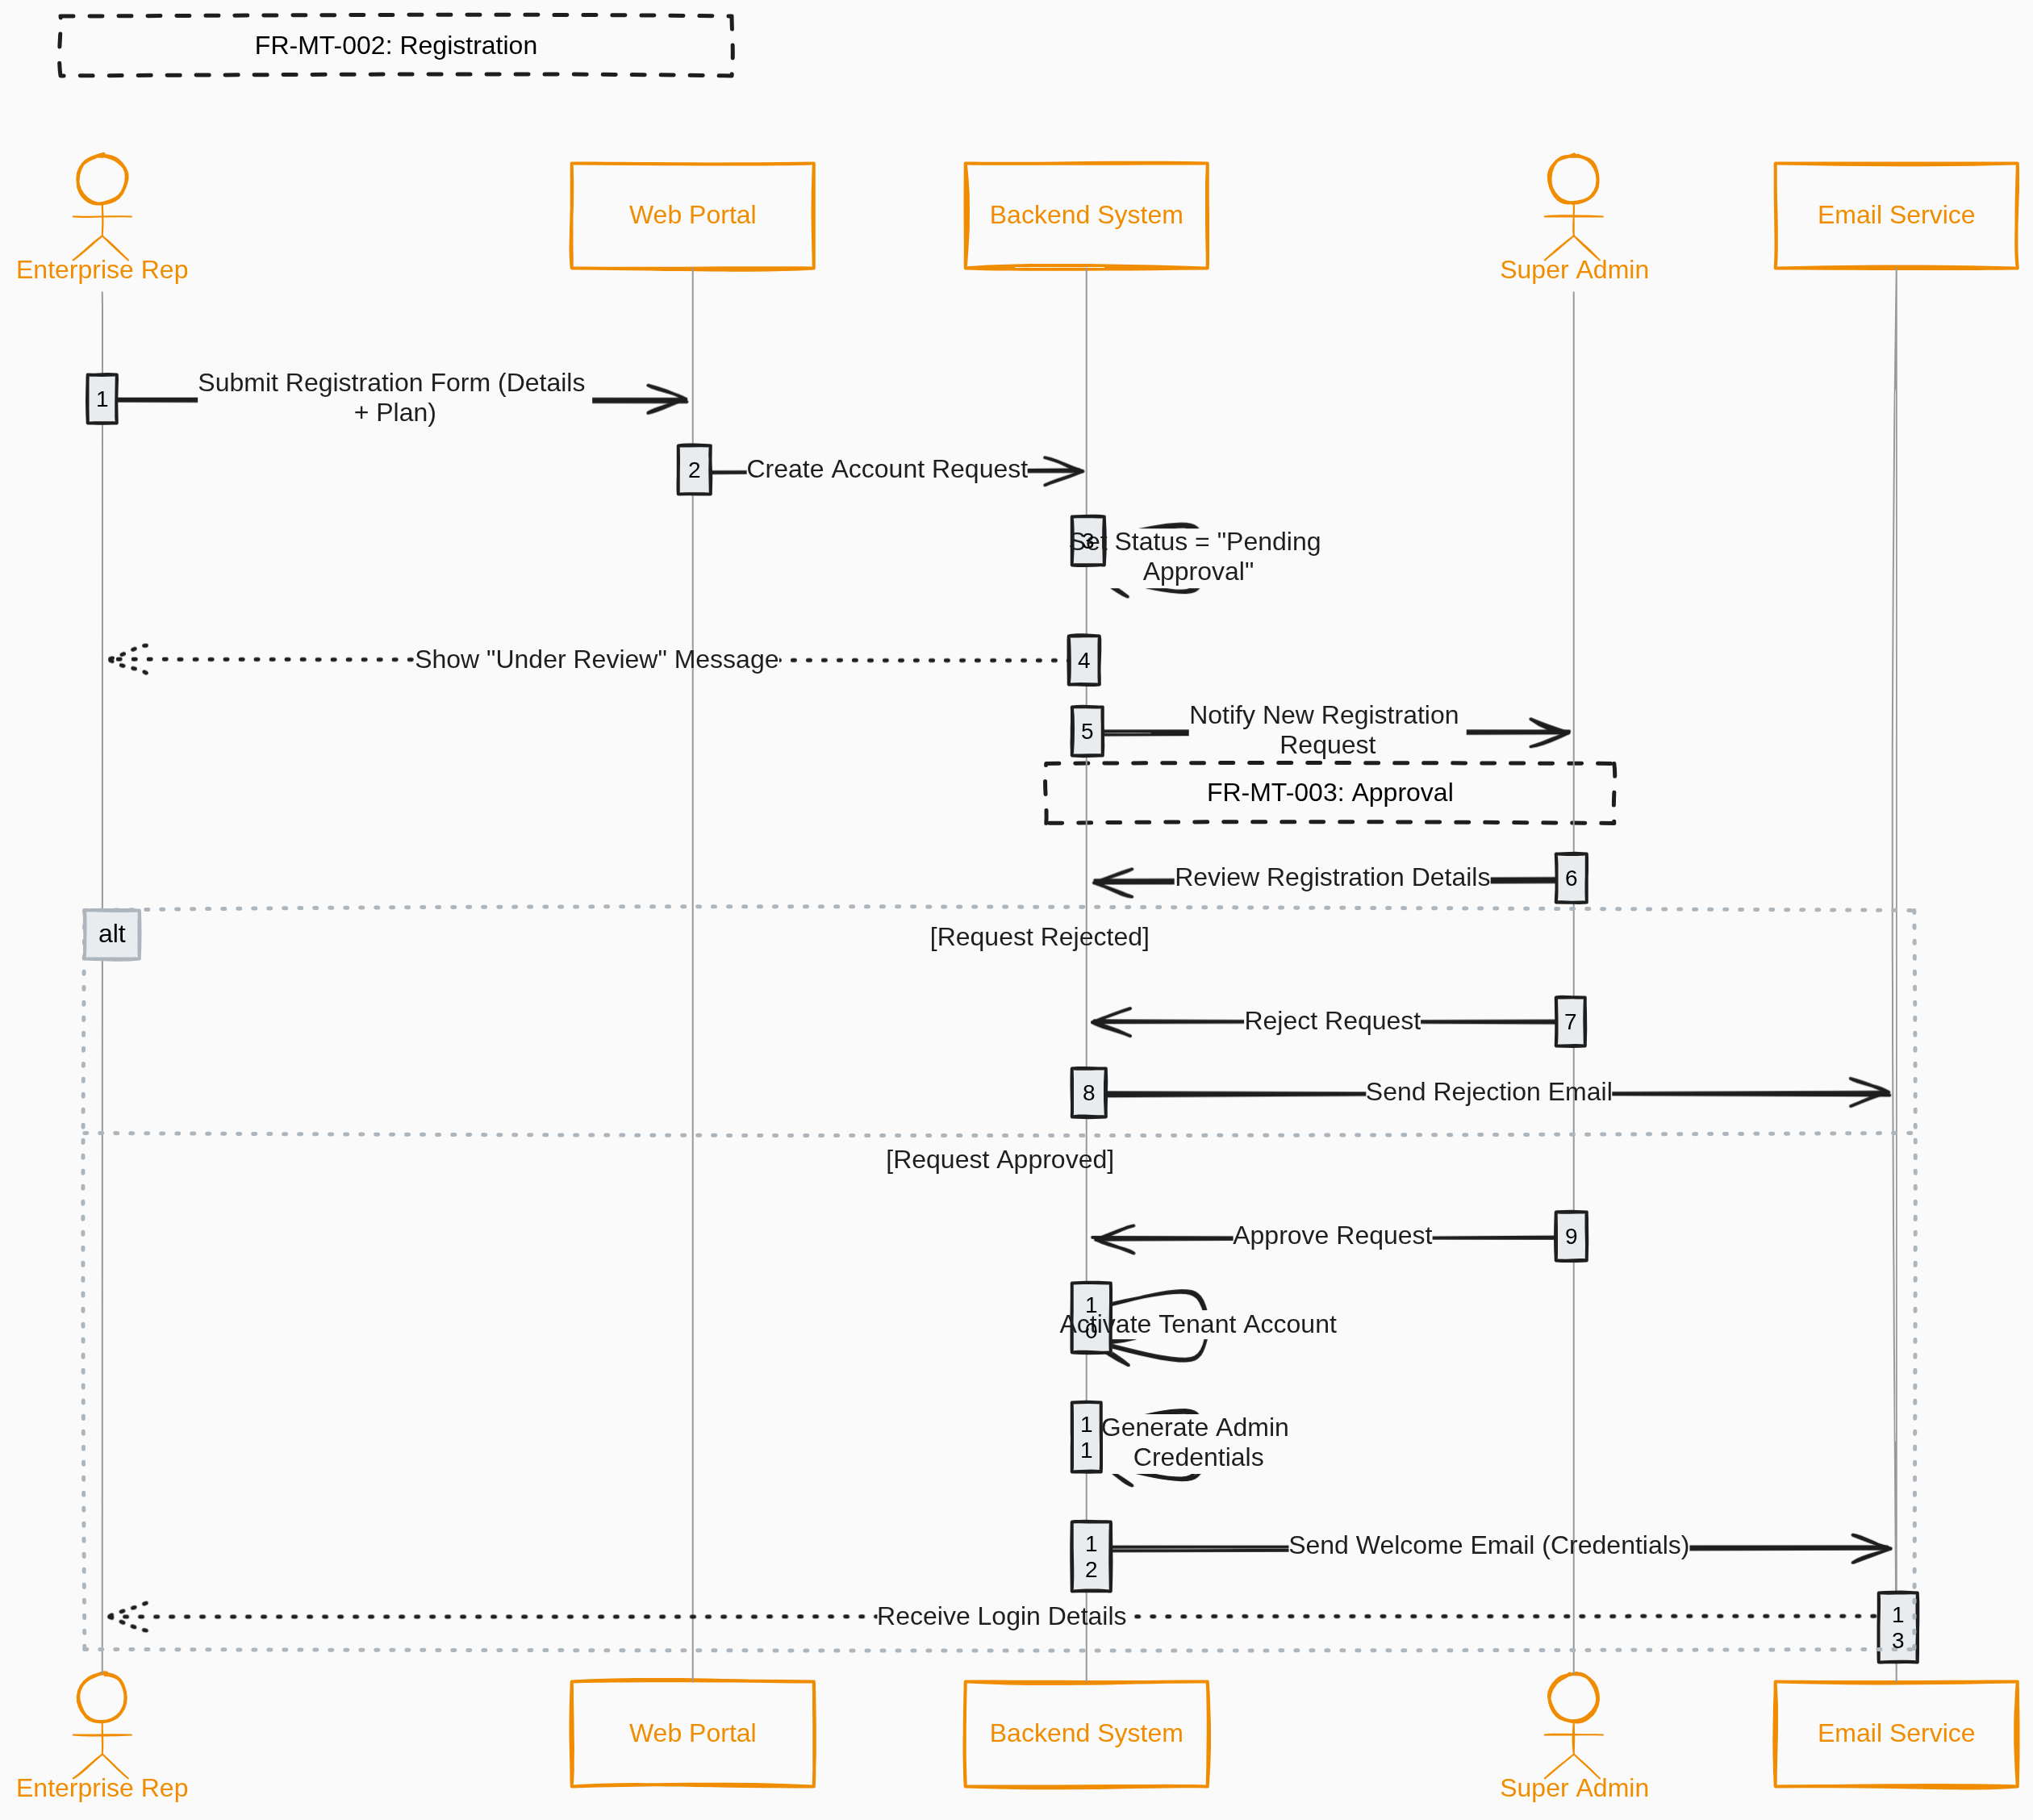
\includegraphics[width=1\linewidth,keepaspectratio]{assets/seq_diagrams/Enterprise Registration.png}
        \caption{Enterprise Registration and Approval Workflow Sequence Diagram}
        \label{fig:enterprise-registration-approval}
        \end{figure}

        \item \textbf{Subscription Payment \& Dunning Process:} This diagram outlines the financial lifecycle of an enterprise account (FR-PAY-004, FR-PAY-008). It shows the billing scheduler triggering a payment request via the gateway (e.g., Telebirr/Stripe). If a transaction fails, the system enters a "Dunning" state, initiating a retry loop and notifying the Enterprise Admin. If all retries fail within the grace period, the account status is automatically set to "Suspended," locking access to protect revenue.
        \vspace*{0.5em}
        \begin{figure}[H]
        \centering
        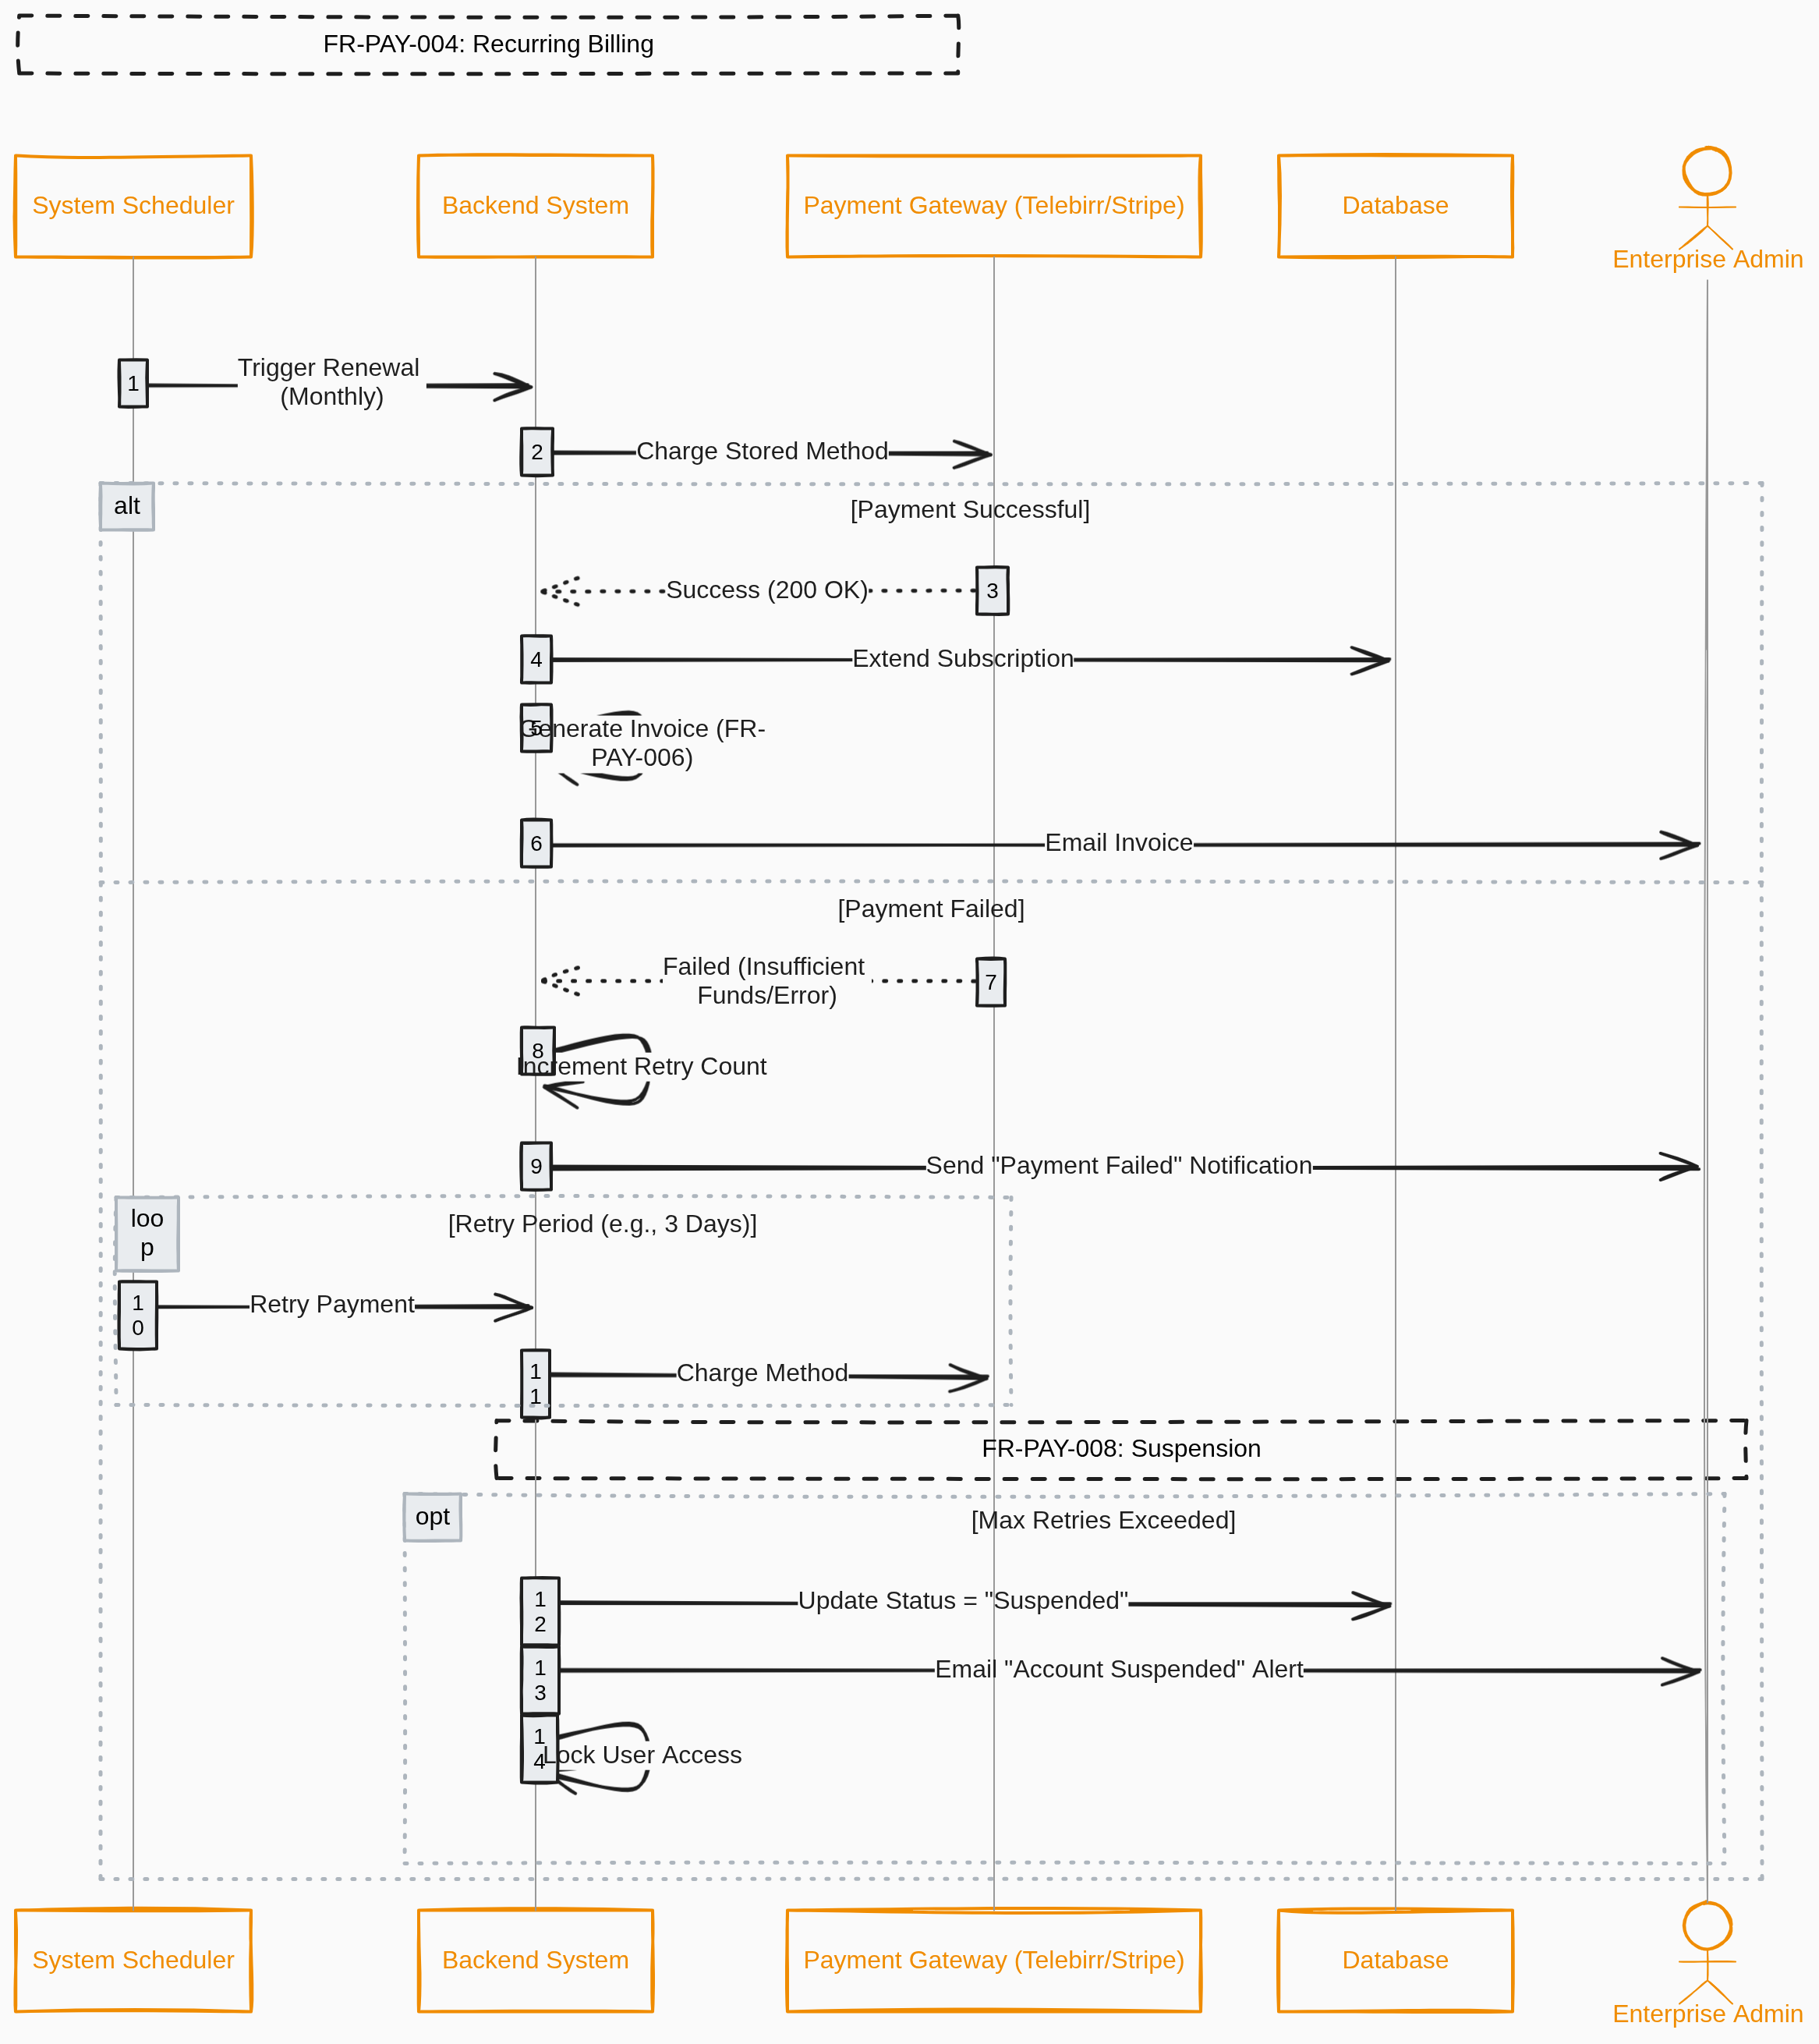
\includegraphics[width=1\linewidth,keepaspectratio]{assets/seq_diagrams/Subscription Payment & Dunning (Suspension).png}
        \caption{Subscription Payment and Dunning Process Sequence Diagram}
        \label{fig:subscription-payment-dunning}
        \end{figure}
        \end{itemize}

    \item \textbf{Authentication \& Security}
        \begin{itemize}
        \item \textbf{Candidate Login with Face Verification:} This diagram visualizes the multi-factor authentication process designed to eliminate impersonation (FR-AUTH-002, FR-AUTH-005). The sequence begins with the candidate entering a unique exam token. Upon validation, the browser interfaces with the webcam to capture a live facial image. This biometric data is transmitted to the backend AI service, which generates a facial vector for registration or verification against an existing profile. Only after the AI service confirms a match or successful registration does the system unlock the exam session, establishing a chain of custody for the candidate's identity.
        \vspace*{0.5em}
        \begin{figure}[H]
        \centering
        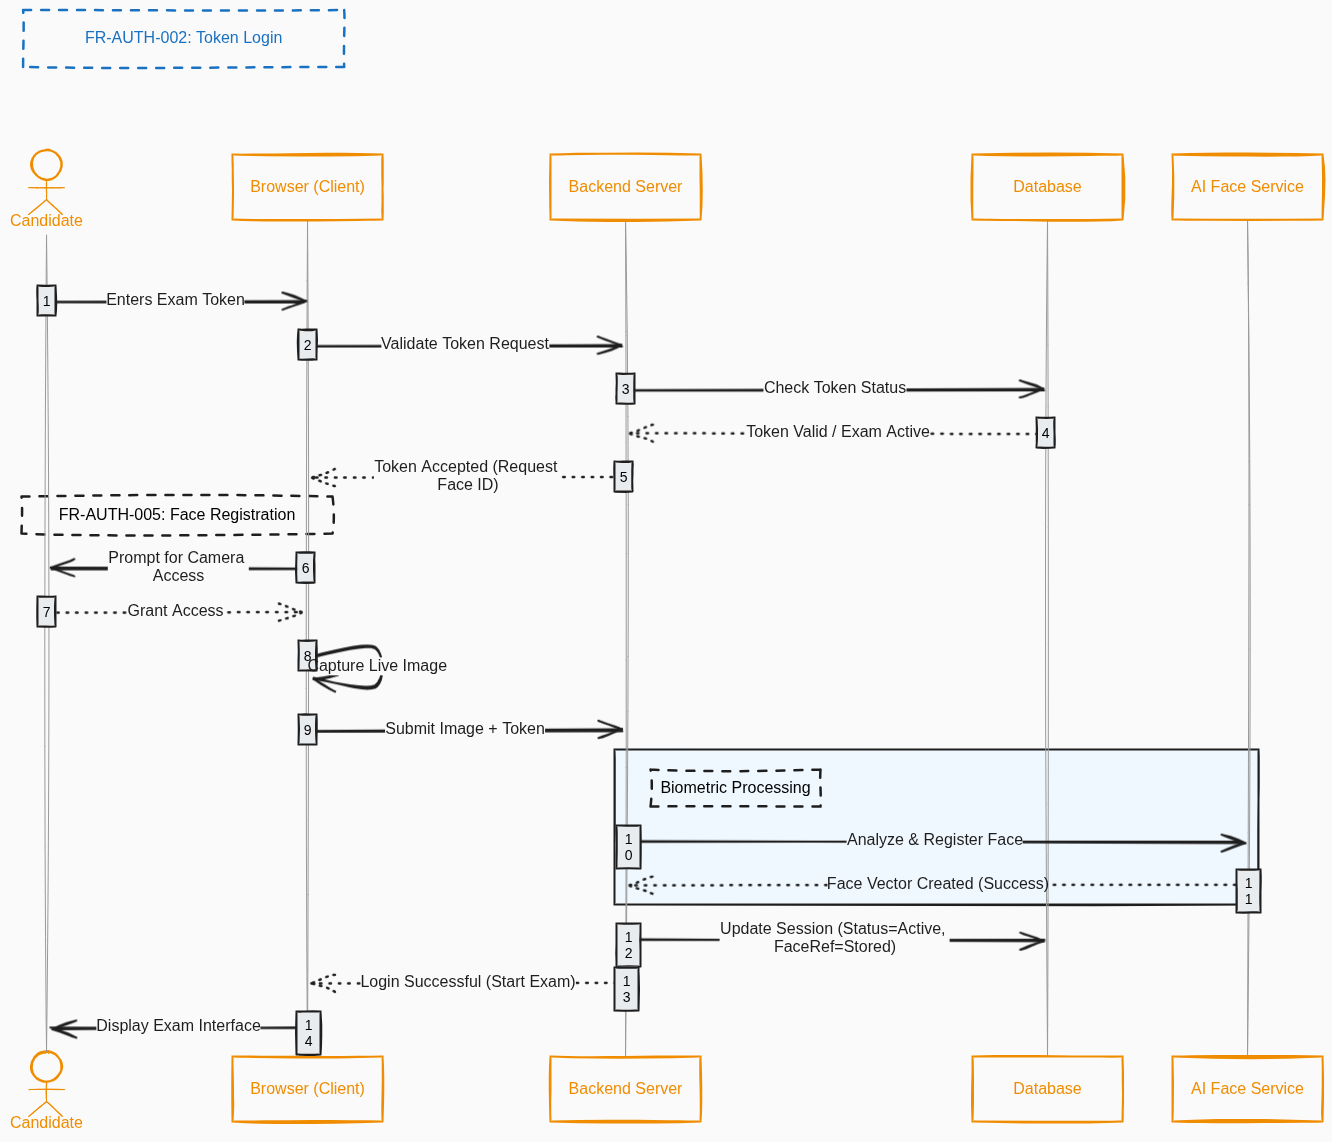
\includegraphics[width=1\linewidth,keepaspectratio]{assets/seq_diagrams/FR-2.png}
        \caption{Candidate Login with Face Verification Sequence Diagram}
        \label{fig:mfa-workflow}
        \end{figure}

        \item \textbf{Session Timeout \& Re-authentication:} \begin{sloppypar}
        This workflow demonstrates the system's security response to user inactivity (FR-AUTH-007). It shows the client-side timer monitoring user interaction; once the idle threshold is breached, the interface is locked (blurred), and the session is paused server-side. The diagram highlights the restoration process, where the candidate must actively request to resume and re-verify their credentials (or face ID). This ensures that an unattended workstation cannot be exploited by a third party during an active exam.
        \end{sloppypar}
        \vspace*{0.5em}
        \begin{figure}[H]
        \centering
        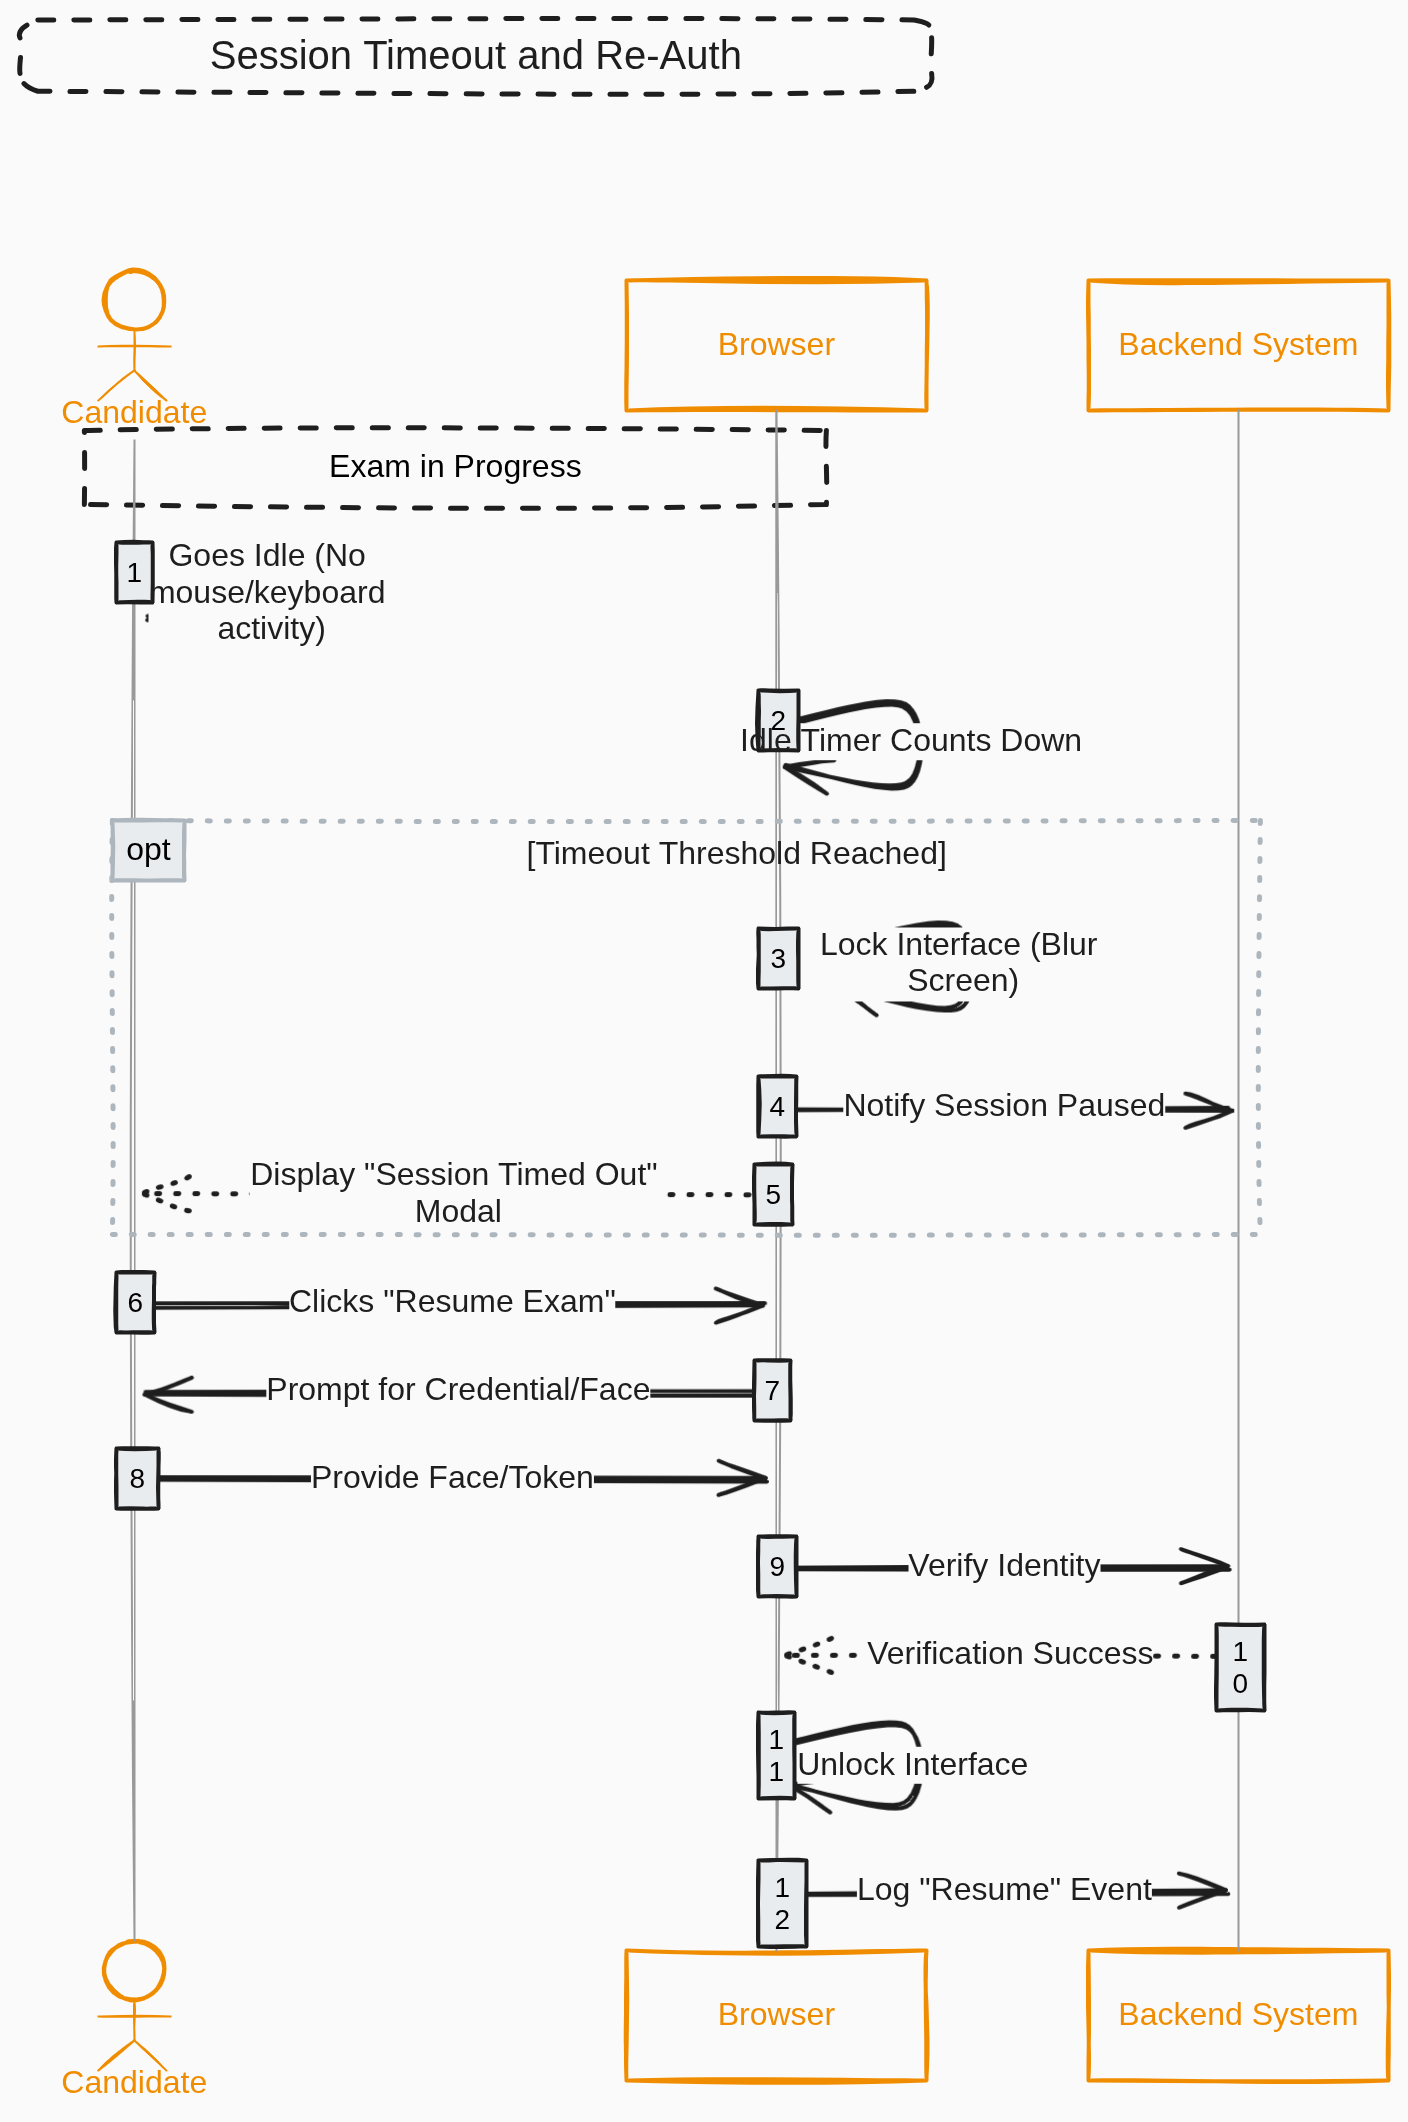
\includegraphics[width=.8\linewidth,keepaspectratio]{assets/seq_diagrams/Session Timeout and Re-Auth.png}
        \caption{Session Timeout and Re-authentication Sequence Diagram}
        \label{fig:session-timeout-reauth}
        \end{figure}
        \end{itemize}
        
    \item \textbf{Examination Management}
        \begin{itemize}
            \item \textbf{Bulk Enrollment \& Token Generation:} This diagram outlines the high-volume data processing required for setting up large exams (FR-EXM-004). It traces the flow from the Enterprise Admin uploading a CSV file to the backend parsing and validating the data against unique constraints (e.g., preventing duplicate emails). Following successful validation, the system iteratively generates cryptographically secure, unique access tokens for each candidate. The process concludes with an asynchronous call to the Email Service, which dispatches personalized invitations without blocking the Admin's user interface.
            \vspace*{0.5em}
            \begin{figure}[H]
            \centering
            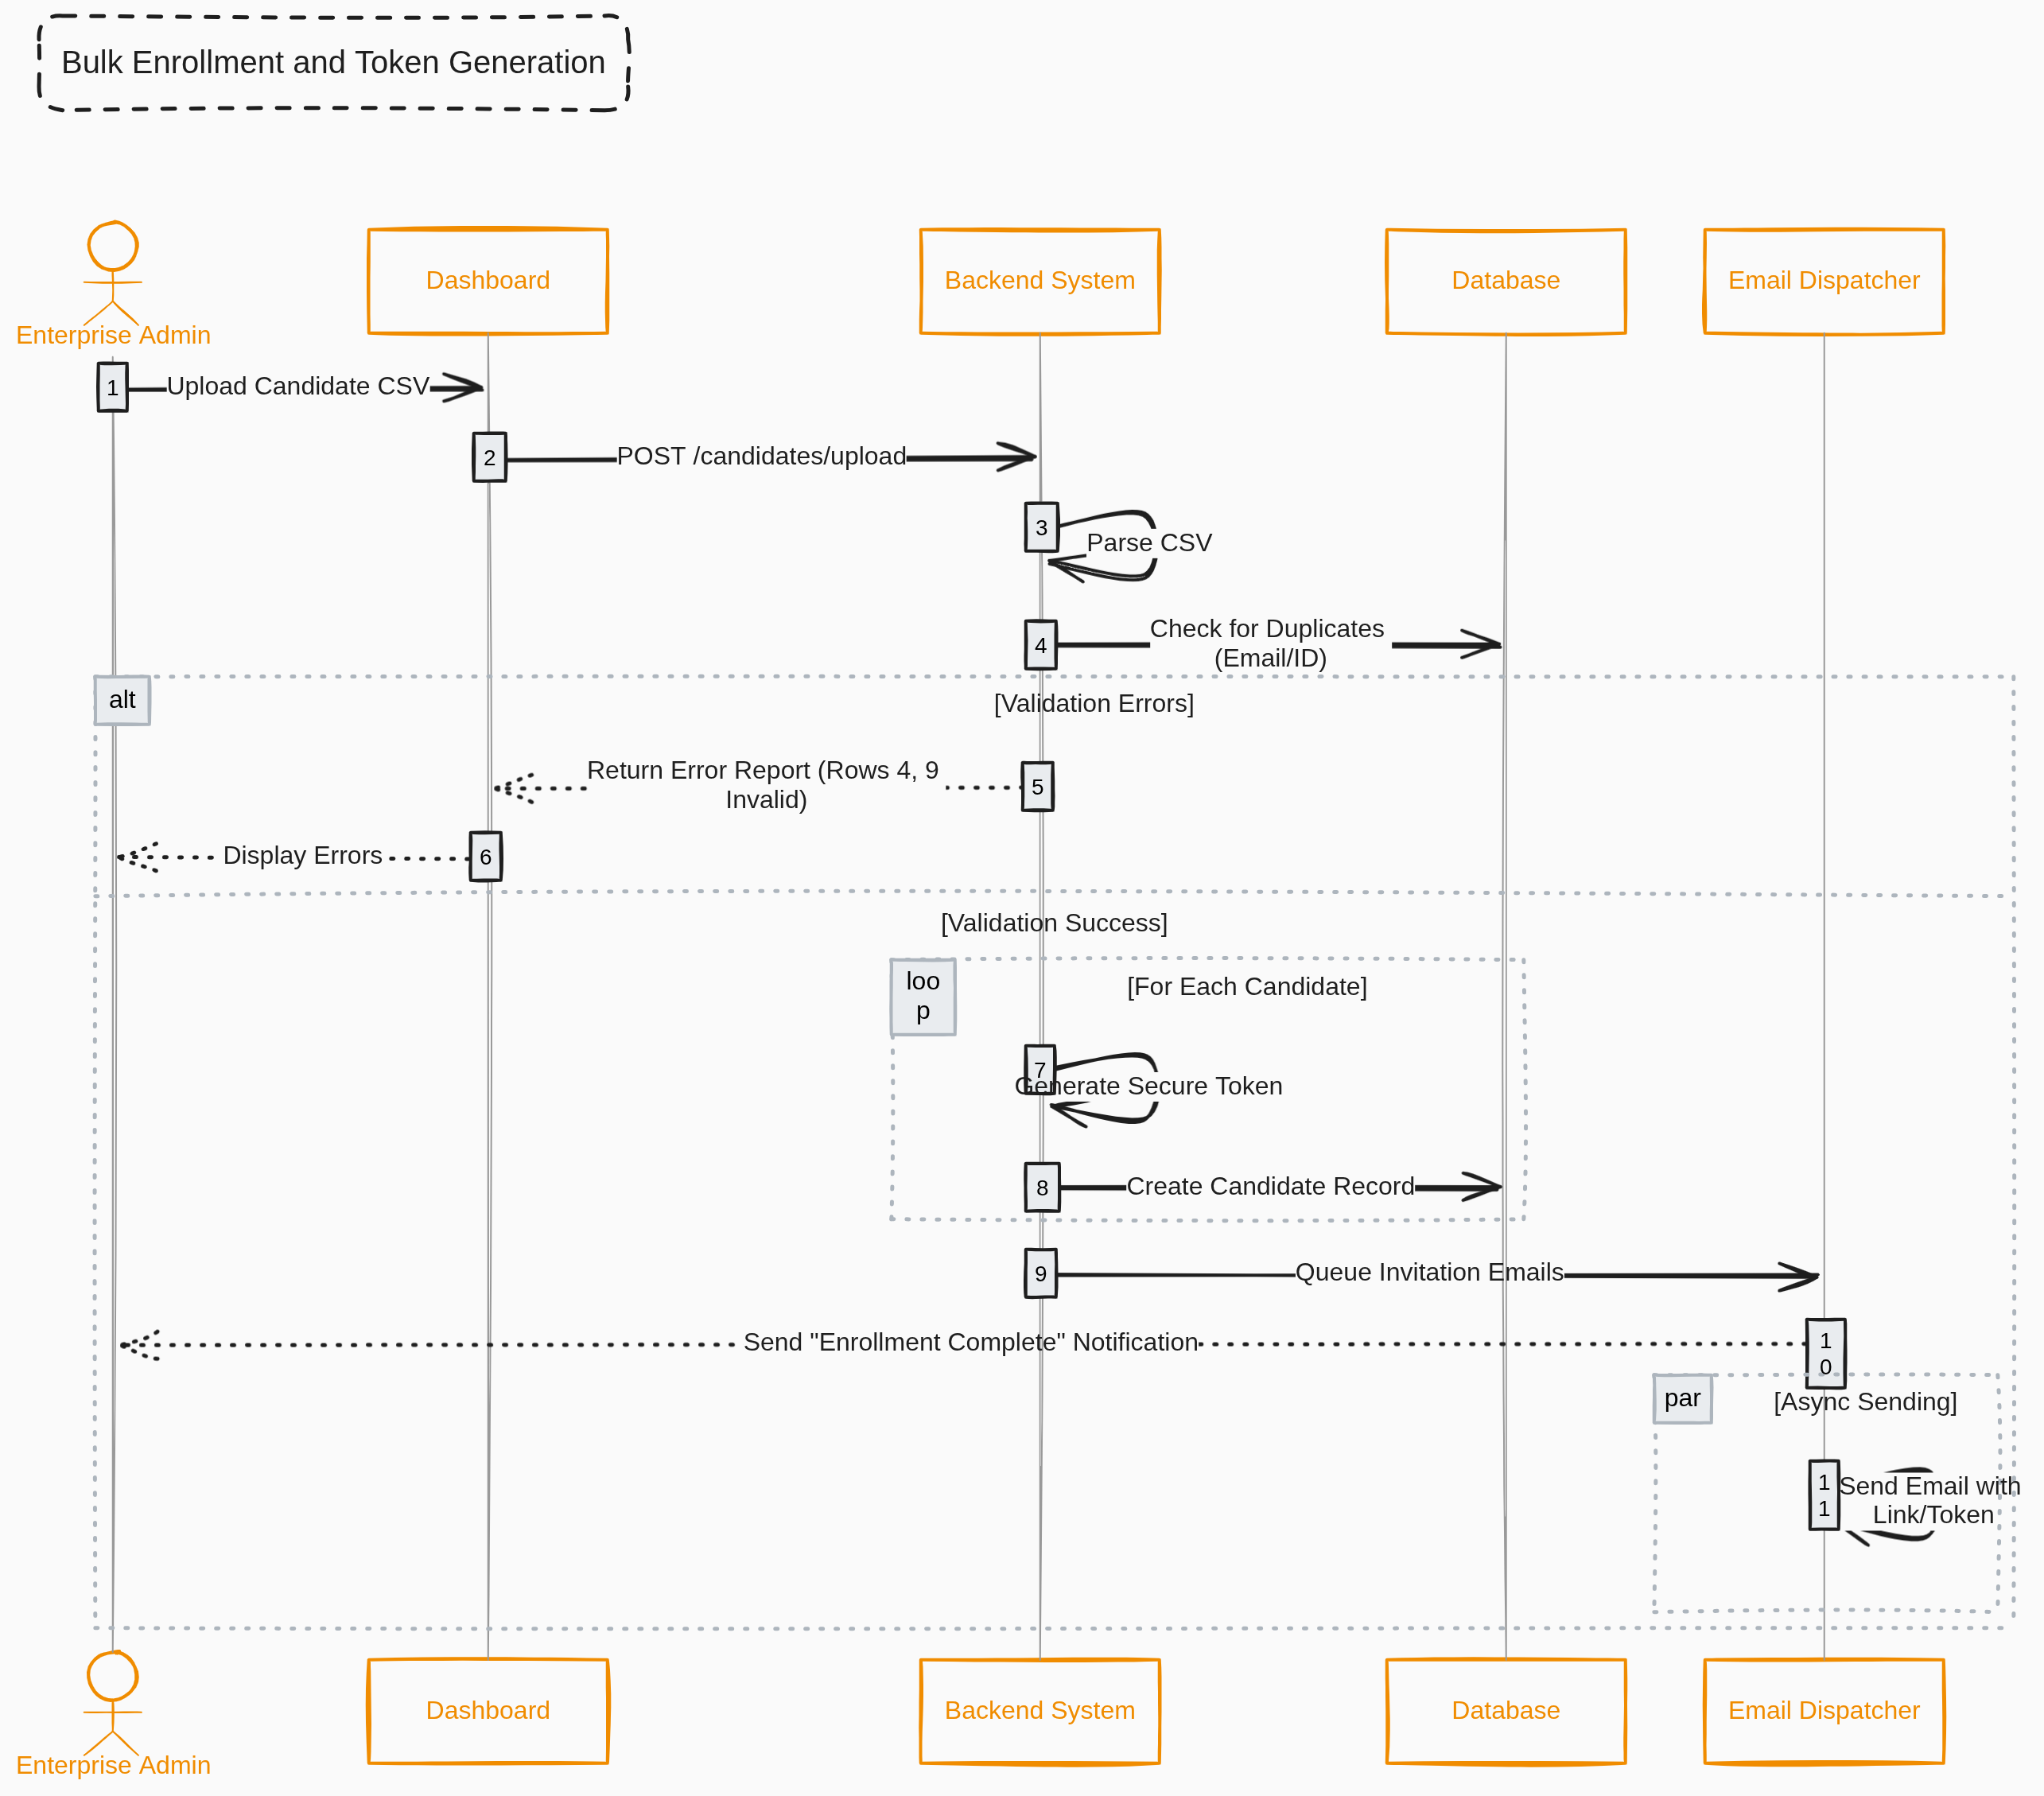
\includegraphics[width=1\linewidth,keepaspectratio]{assets/seq_diagrams/Bulk Enrollment and Token Gen.png}
            \caption{Bulk Enrollment and Token Generation Sequence Diagram}
            \label{fig:bulk-enrollment-token-generation}
            \end{figure}

            \item \textbf{Exam Configuration (Targeted Randomization):} This diagram explains the logic behind creating dynamic, randomized exams (FR-EXM-002). It depicts the interaction between the Admin's configuration wizard and the Question Bank database. When an Admin defines complex criteria (e.g., "5 Hard questions from Topic A"), the system performs a validation query to ensure sufficient questions exist in the bank. Once validated, the system saves the structure or template of the exam rather than a fixed list of questions, enabling the runtime engine to generate a unique question set for every candidate.
            \vspace*{0.5em}
            \begin{figure}[H]
            \centering
            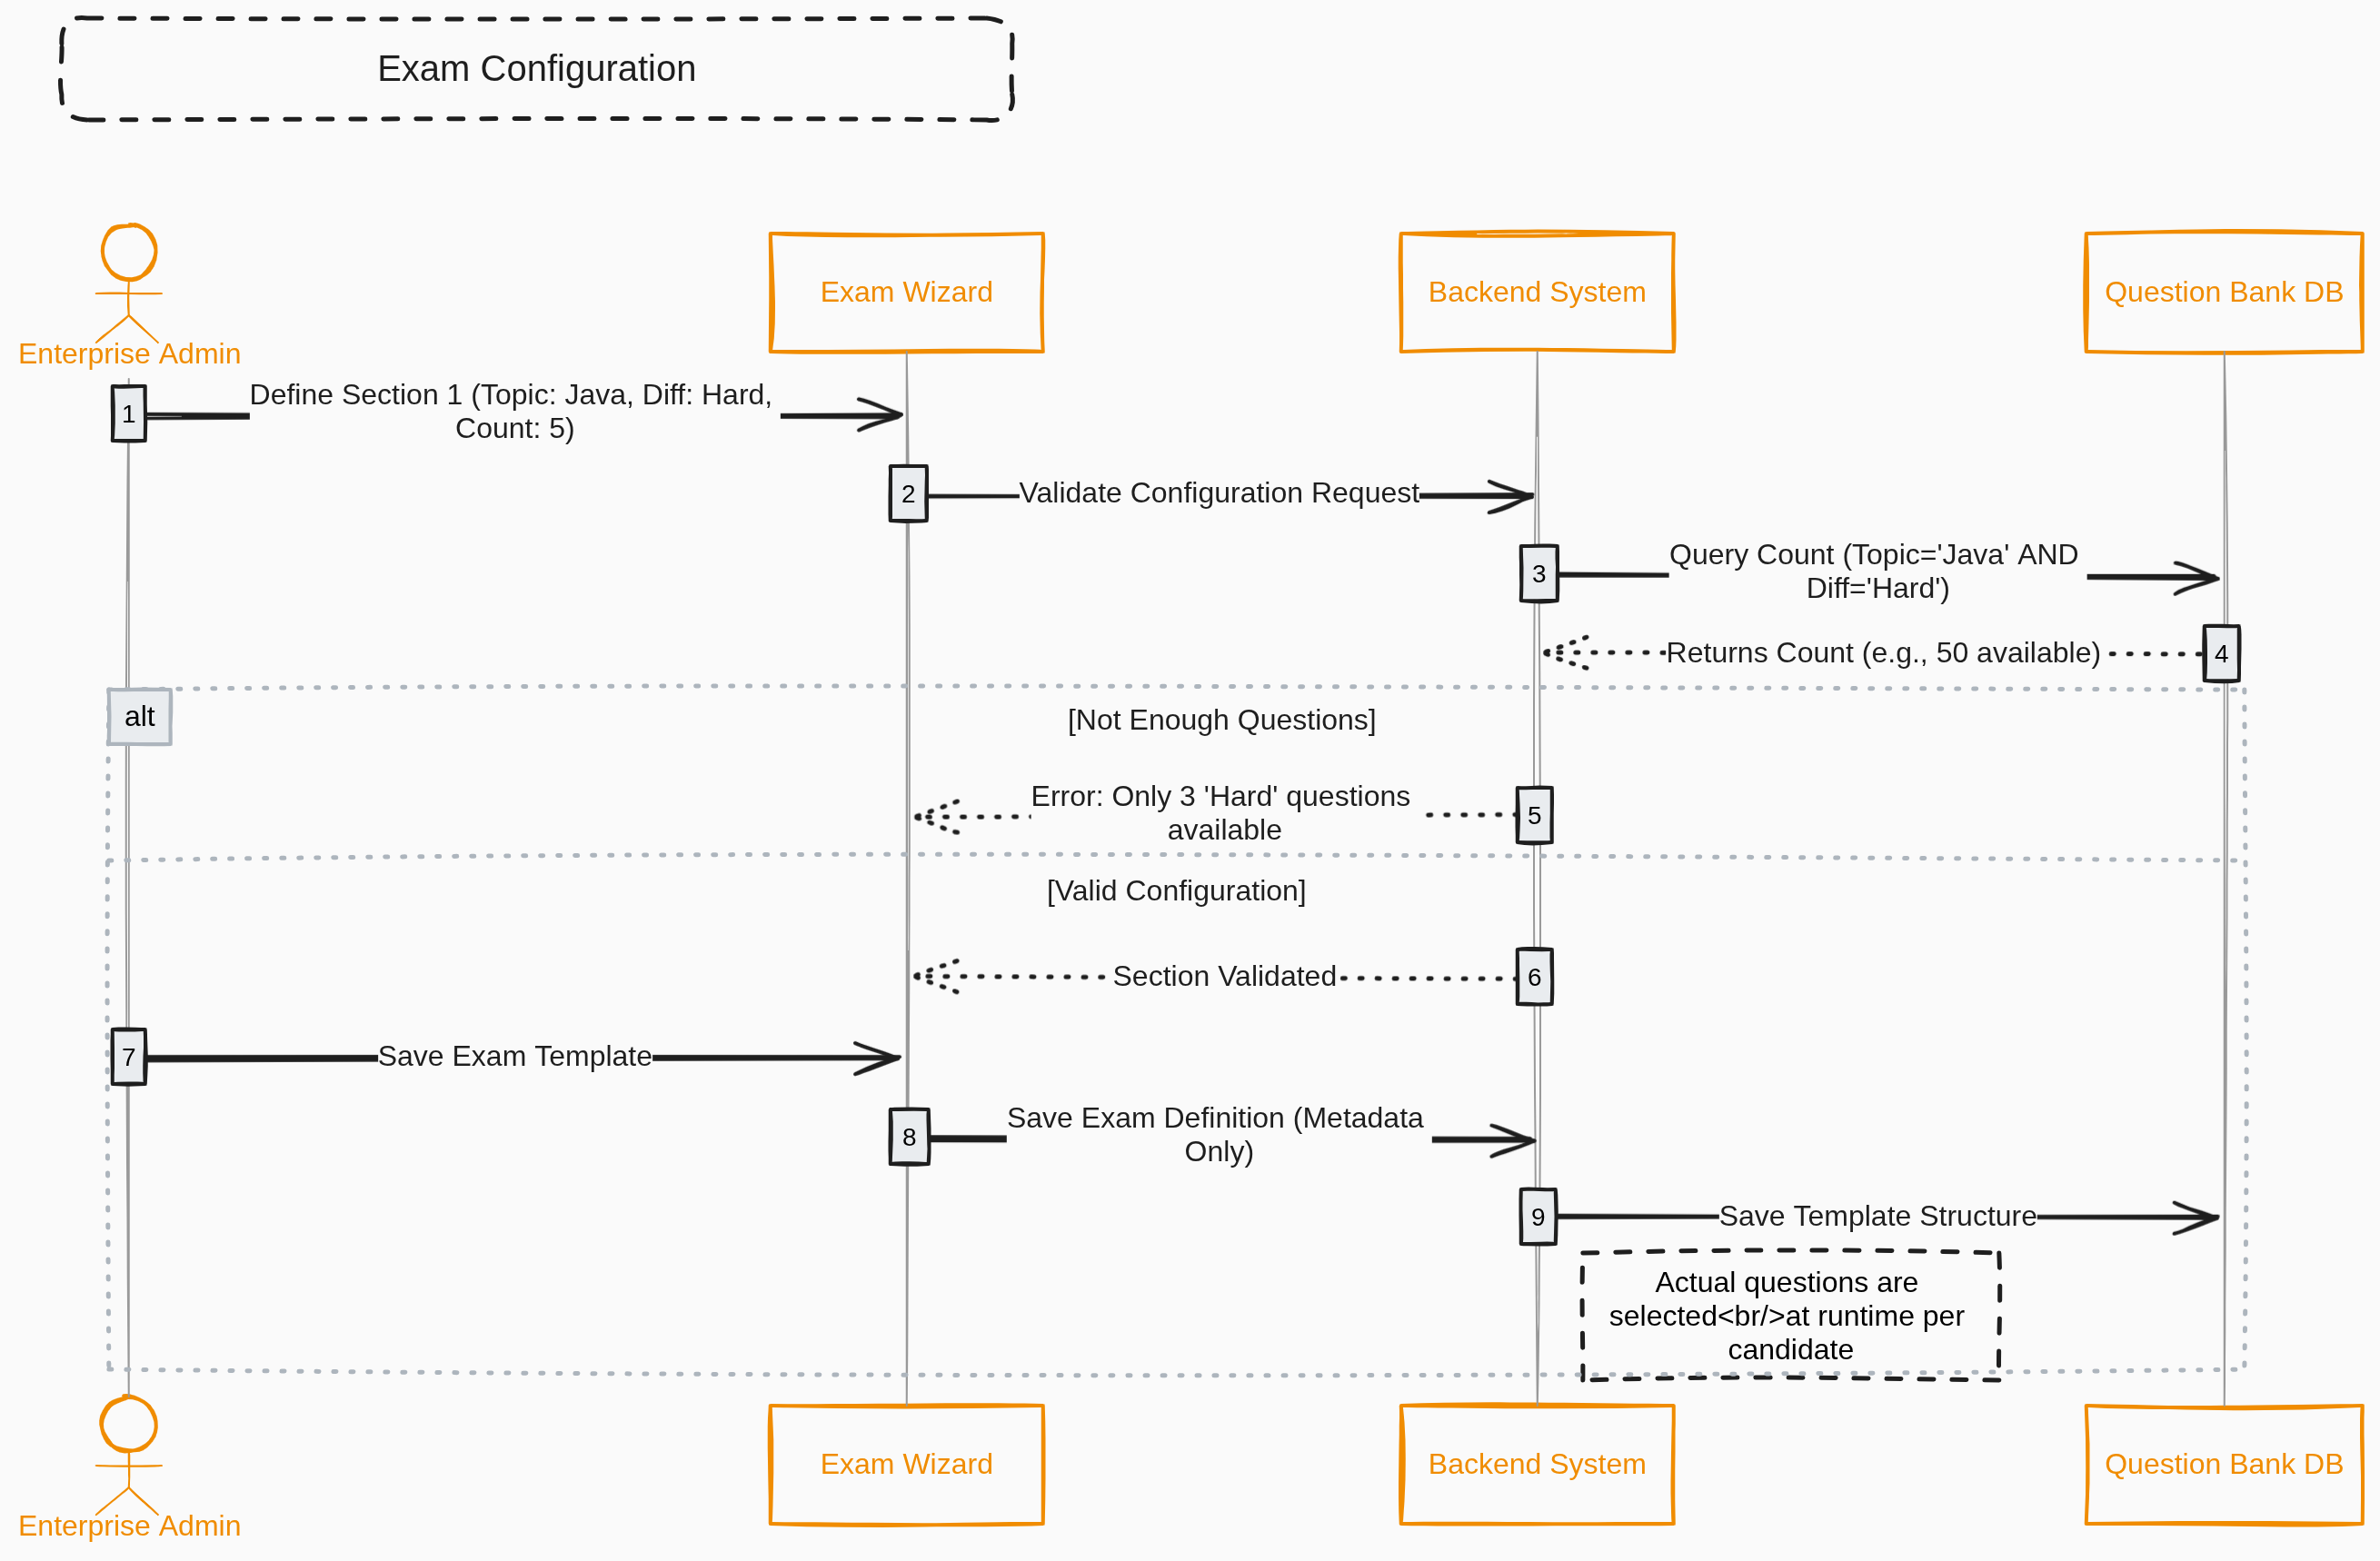
\includegraphics[width=1\linewidth,keepaspectratio]{assets/seq_diagrams/Exam Configuration.png}
            \caption{Exam Configuration (Targeted Randomization) Sequence Diagram}
            \label{fig:exam-configuration-randomization}
            \end{figure}
        \end{itemize}
    
    \item \textbf{Candidate Exam Experience}
        \begin{itemize}
            \item \textbf{Answer Auto-Save \& Sync:} This diagram illustrates the data synchronization mechanism that protects candidate progress (FR-CAND-004). It shows the continuous loop where candidate inputs are first committed to the browser's local storage (IndexedDB) for immediate latency-free feedback. A background timer then periodically triggers a synchronization event, pushing the local data to the backend server. This "save-forward" approach ensures that a server crash or network hiccup results in minimal data loss, as the "truth" is maintained in two locations.
            \vspace*{0.5em}
            \begin{figure}[H]
            \centering
            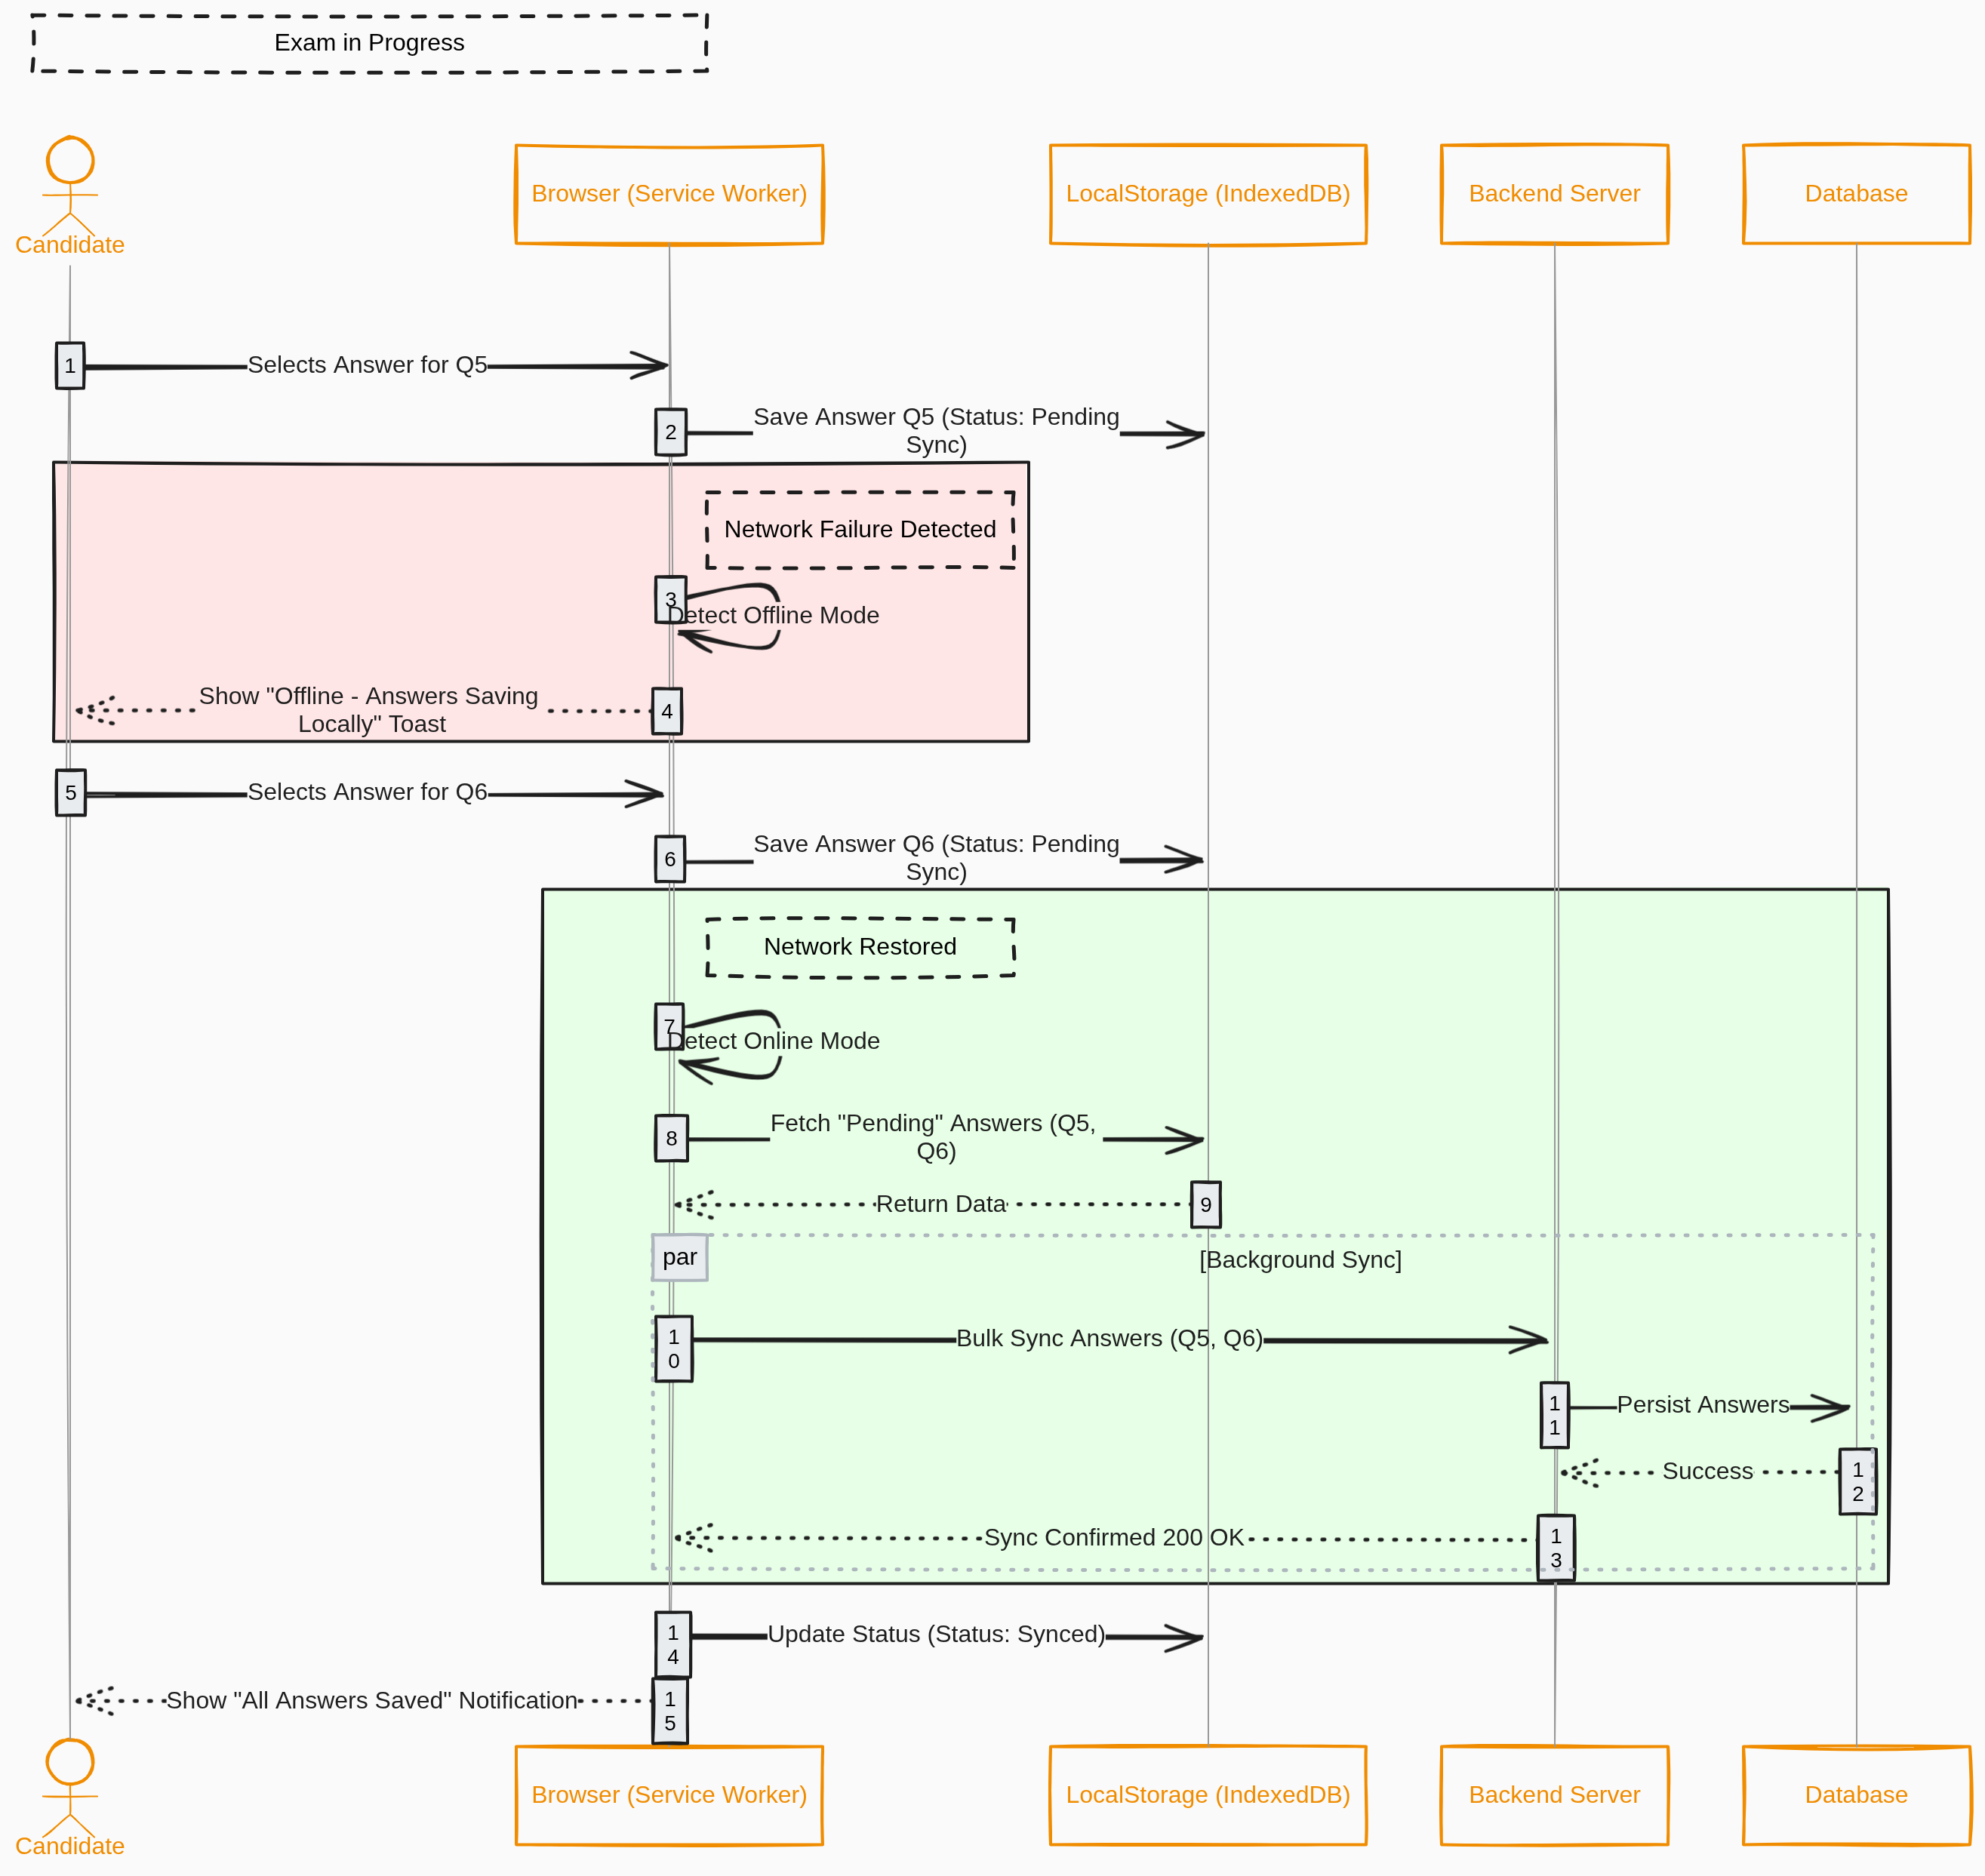
\includegraphics[width=1\linewidth,keepaspectratio]{assets/seq_diagrams/Exam in Progress.png}
            \caption{Answer Auto-Save and Sync Sequence Diagram}
            \label{fig:answer-auto-save-sync}
            \end{figure}
        \end{itemize}
    
    \item \textbf{AI Proctoring \& Monitoring}
        \begin{itemize}
            \item \textbf{Proctoring Event Loop:} This diagram visualizes the real-time monitoring loop that runs throughout the exam (FR-PROC-001, FR-DASH-002). It breaks down parallel processes: the browser detecting OS-level events (like tab switching) and the webcam capturing periodic frames for AI analysis. These inputs are sent to the server, which calculates a cumulative "Cheating Probability Score" based on the frequency and severity of events. The diagram concludes by showing how these flags are pushed via WebSocket to the Admin's Live Dashboard, enabling immediate intervention.
            \vspace*{0.5em}
            \begin{figure}[H]
            \centering
            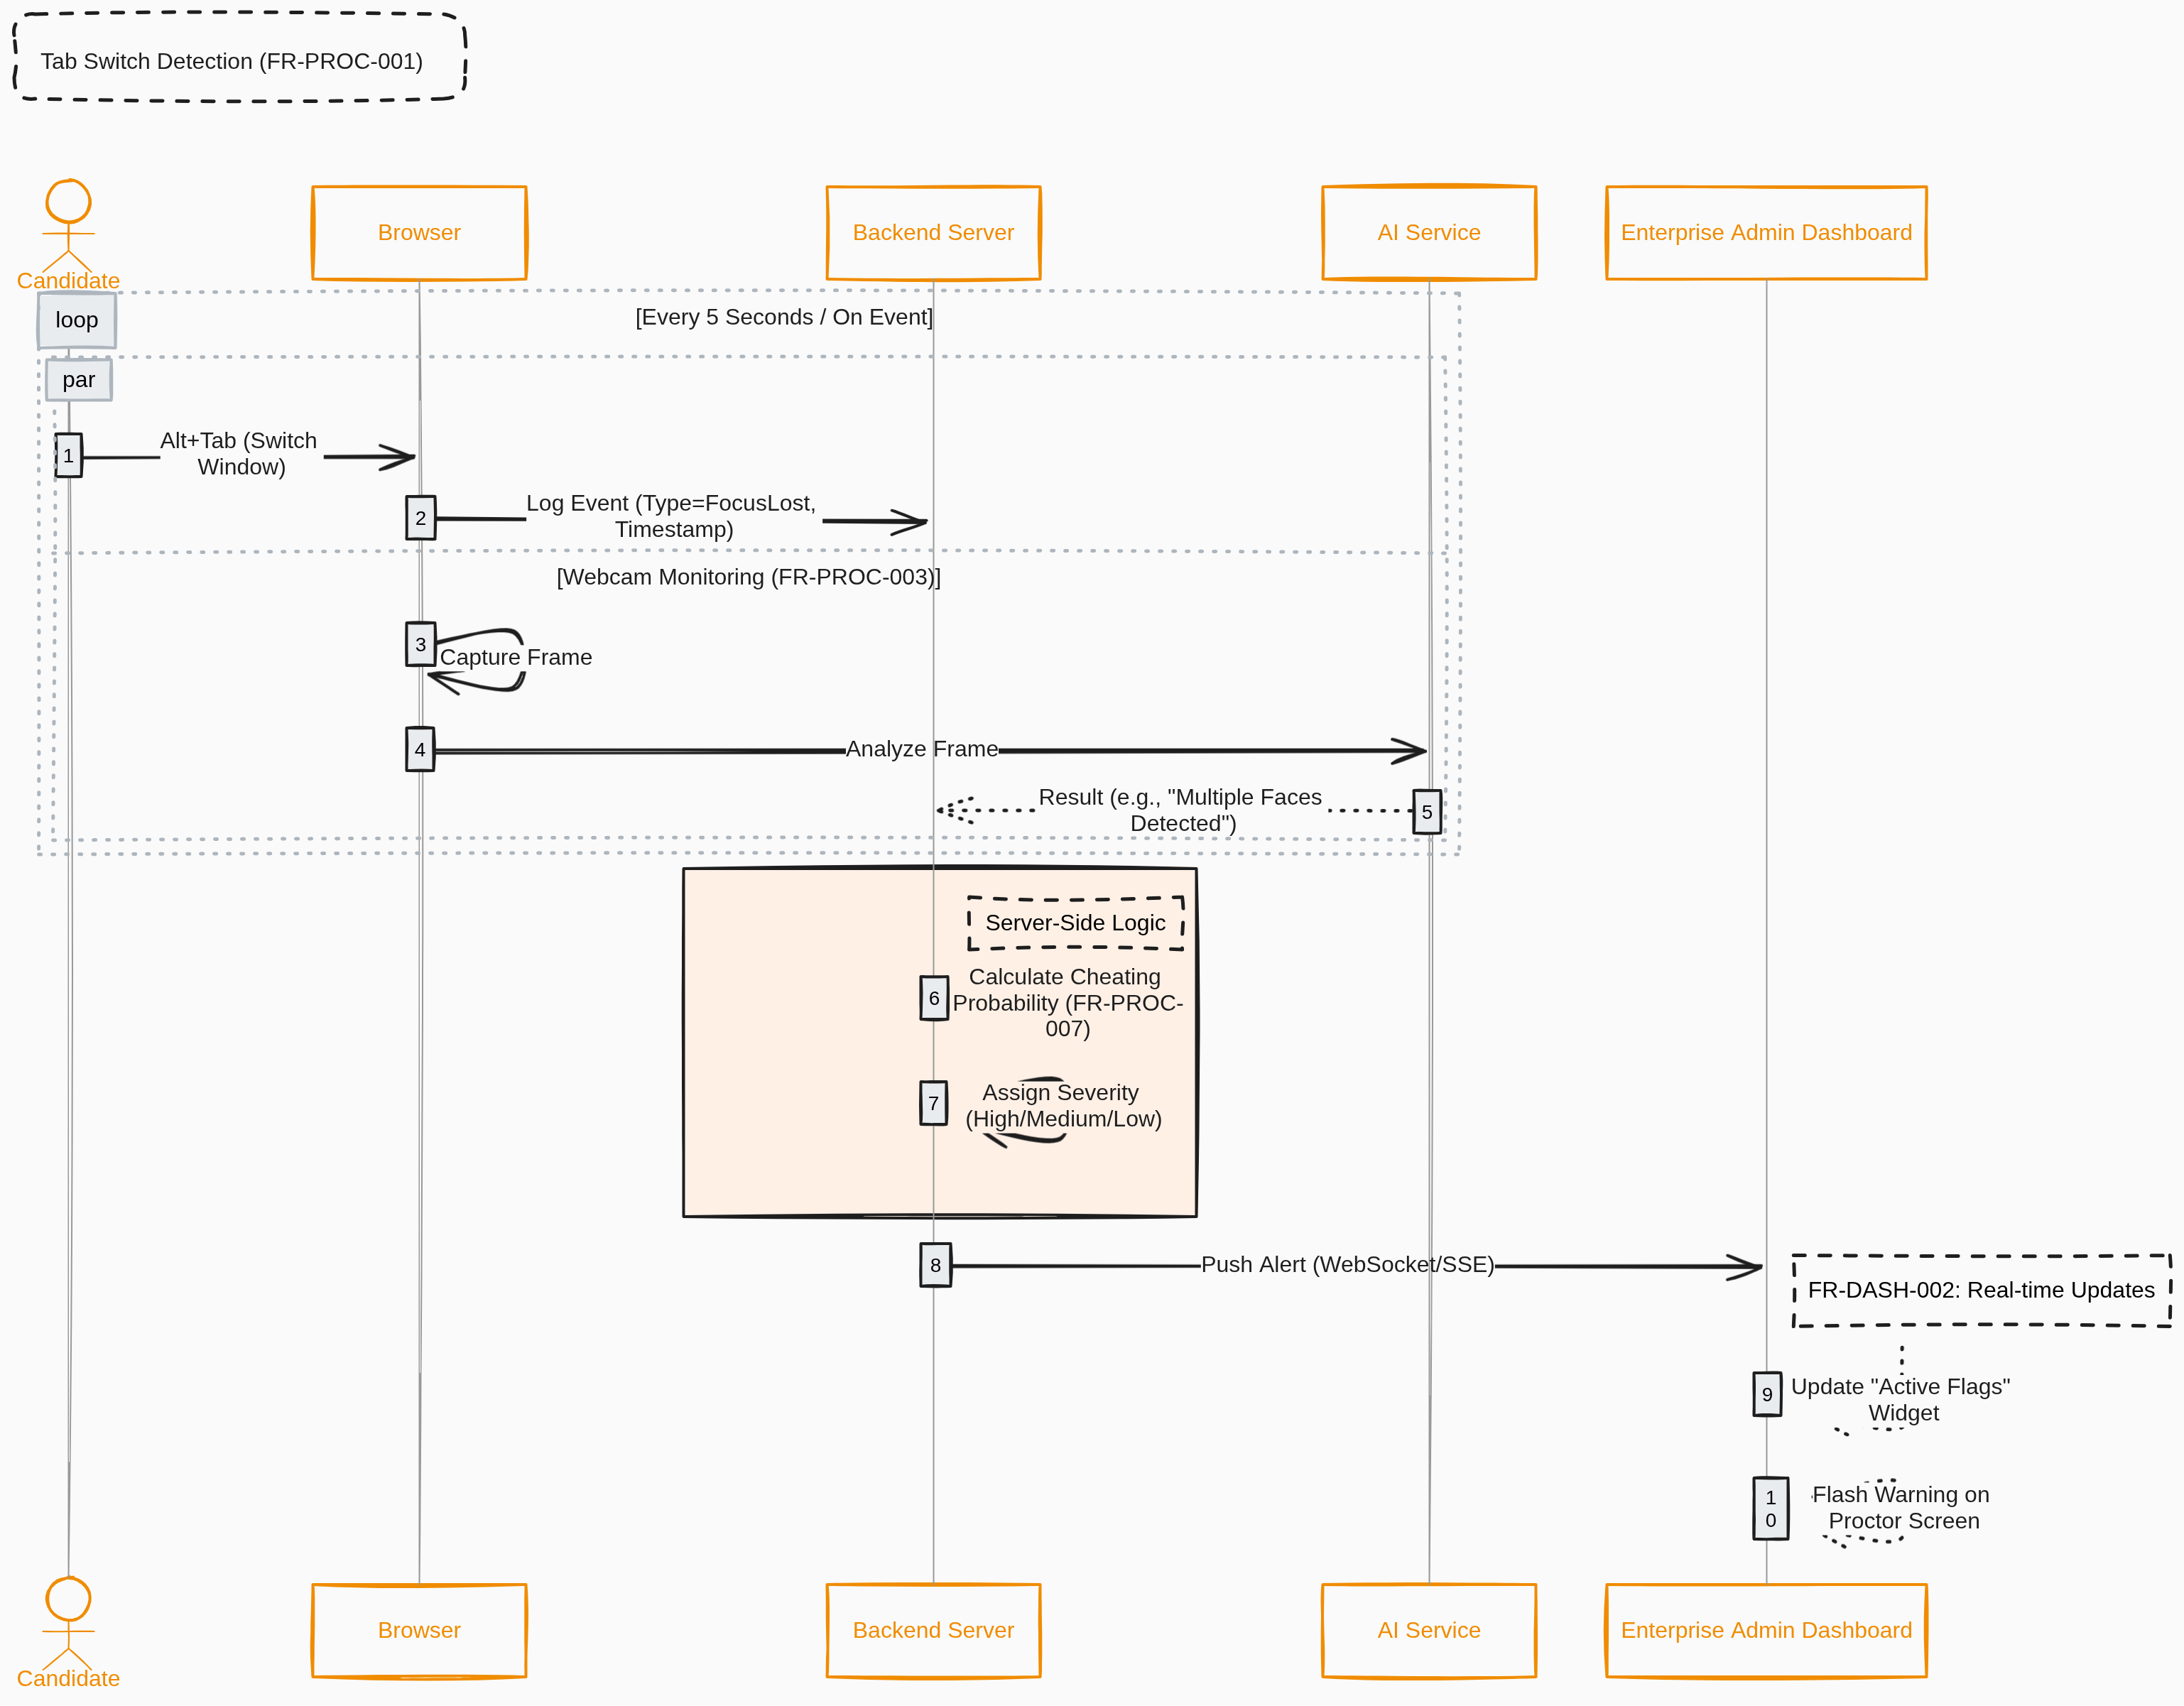
\includegraphics[width=1\linewidth,keepaspectratio]{assets/seq_diagrams/Tab Switch Detection.png}
            \caption{Proctoring Event Loop Sequence Diagram}
            \label{fig:proctoring-event-loop}
            \end{figure}
        \end{itemize}
    
    \item \textbf{Grading \& Reporting}
        \begin{itemize}
            \item \textbf{Hybrid Grading Workflow:} This diagram explains the split-processing logic for mixed-format exams (FR-GRAD-001, FR-GRAD-002). It shows objective answers (MCQ) being routed immediately to the Auto-Grader for instant scoring, while subjective answers (Essays) are queued for human review. Crucially, the diagram highlights the privacy layer where the system strips candidate identifiers before presenting the answer to the Human Reviewer ("Blind Grading"), ensuring the final grade is composed of unbiased manual scores and calculated automated scores.
            \vspace*{0.5em}
            \begin{figure}[H]
            \centering
            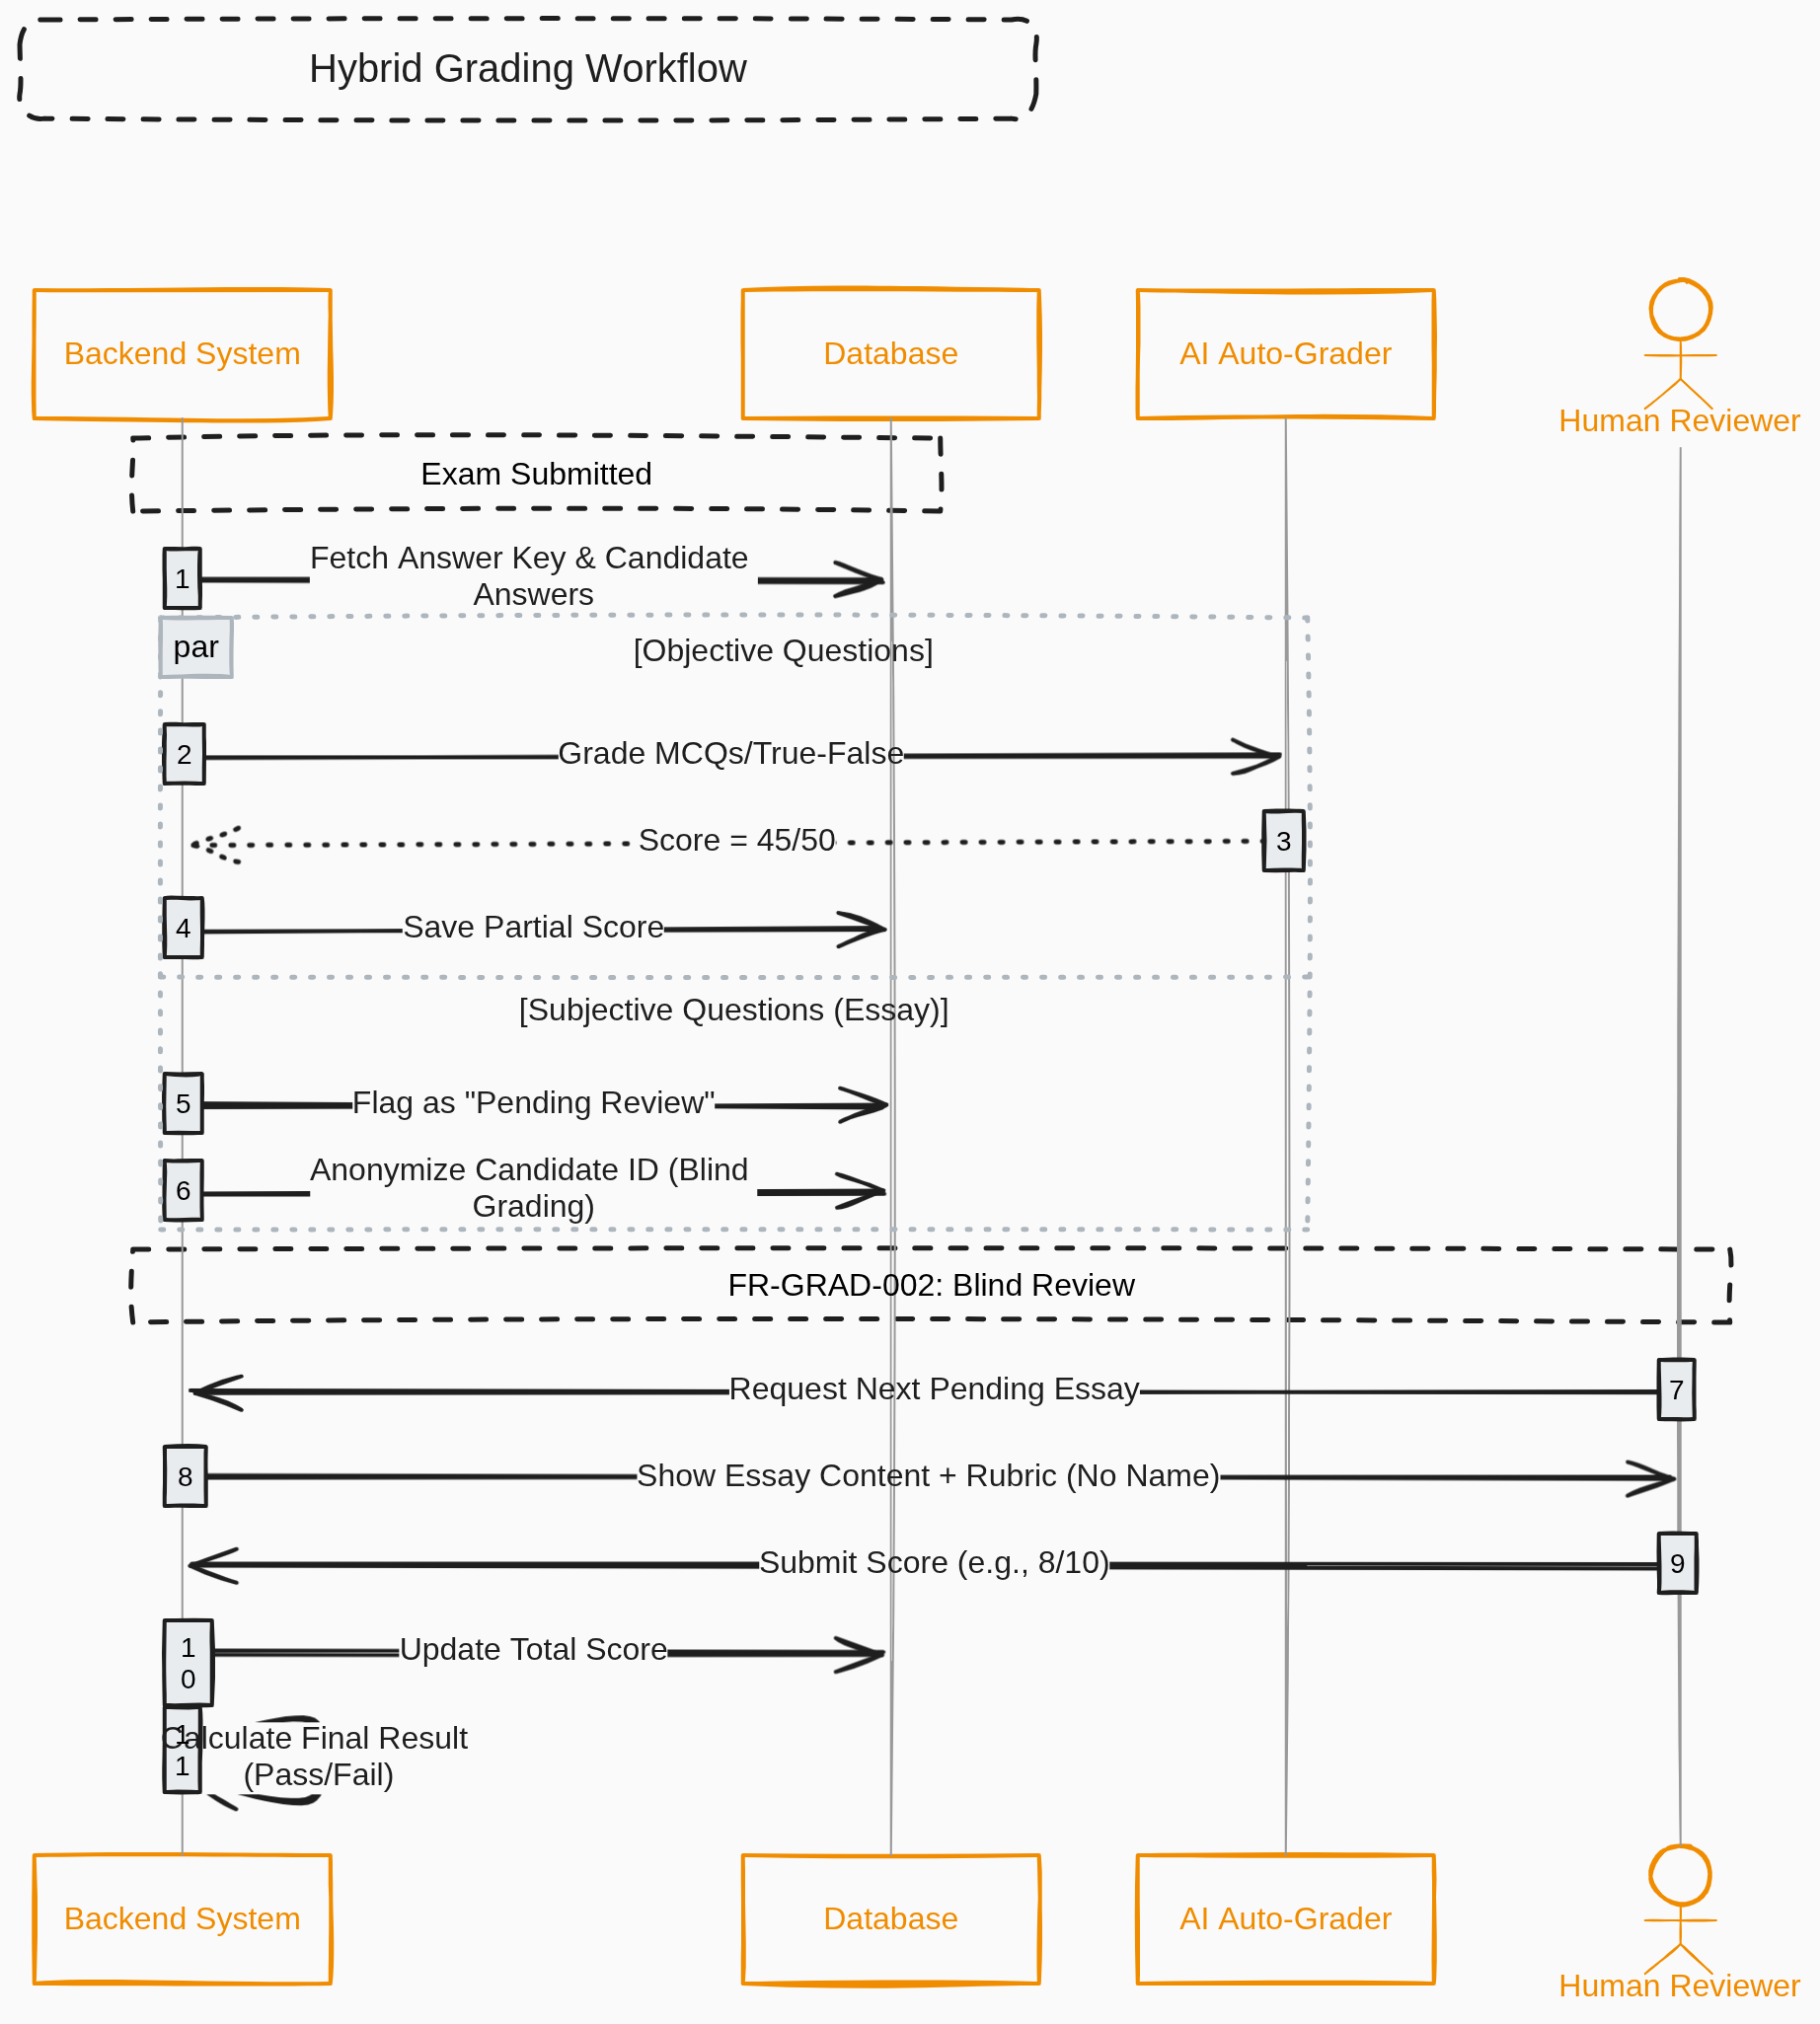
\includegraphics[width=1\linewidth,keepaspectratio]{assets/seq_diagrams/Hybrid Grading Workflow.png}
            \caption{Hybrid Grading Workflow Sequence Diagram}
            \label{fig:hybrid-grading-workflow}
            \end{figure}

            \item \textbf{Async Report Generation:} This diagram addresses system performance during heavy data retrieval operations (FR-DASH-003). It depicts the flow when an Admin requests a large report (e.g., $\geq$500 records). Instead of processing the request synchronously and freezing the browser, the backend offloads the task to a Job Queue. A background Worker Service picks up the job, generates the file, and notifies the user via email or in-app alert when the download is ready, maintaining system responsiveness.
            \vspace*{0.5em}
            \begin{figure}[H]
            \centering
            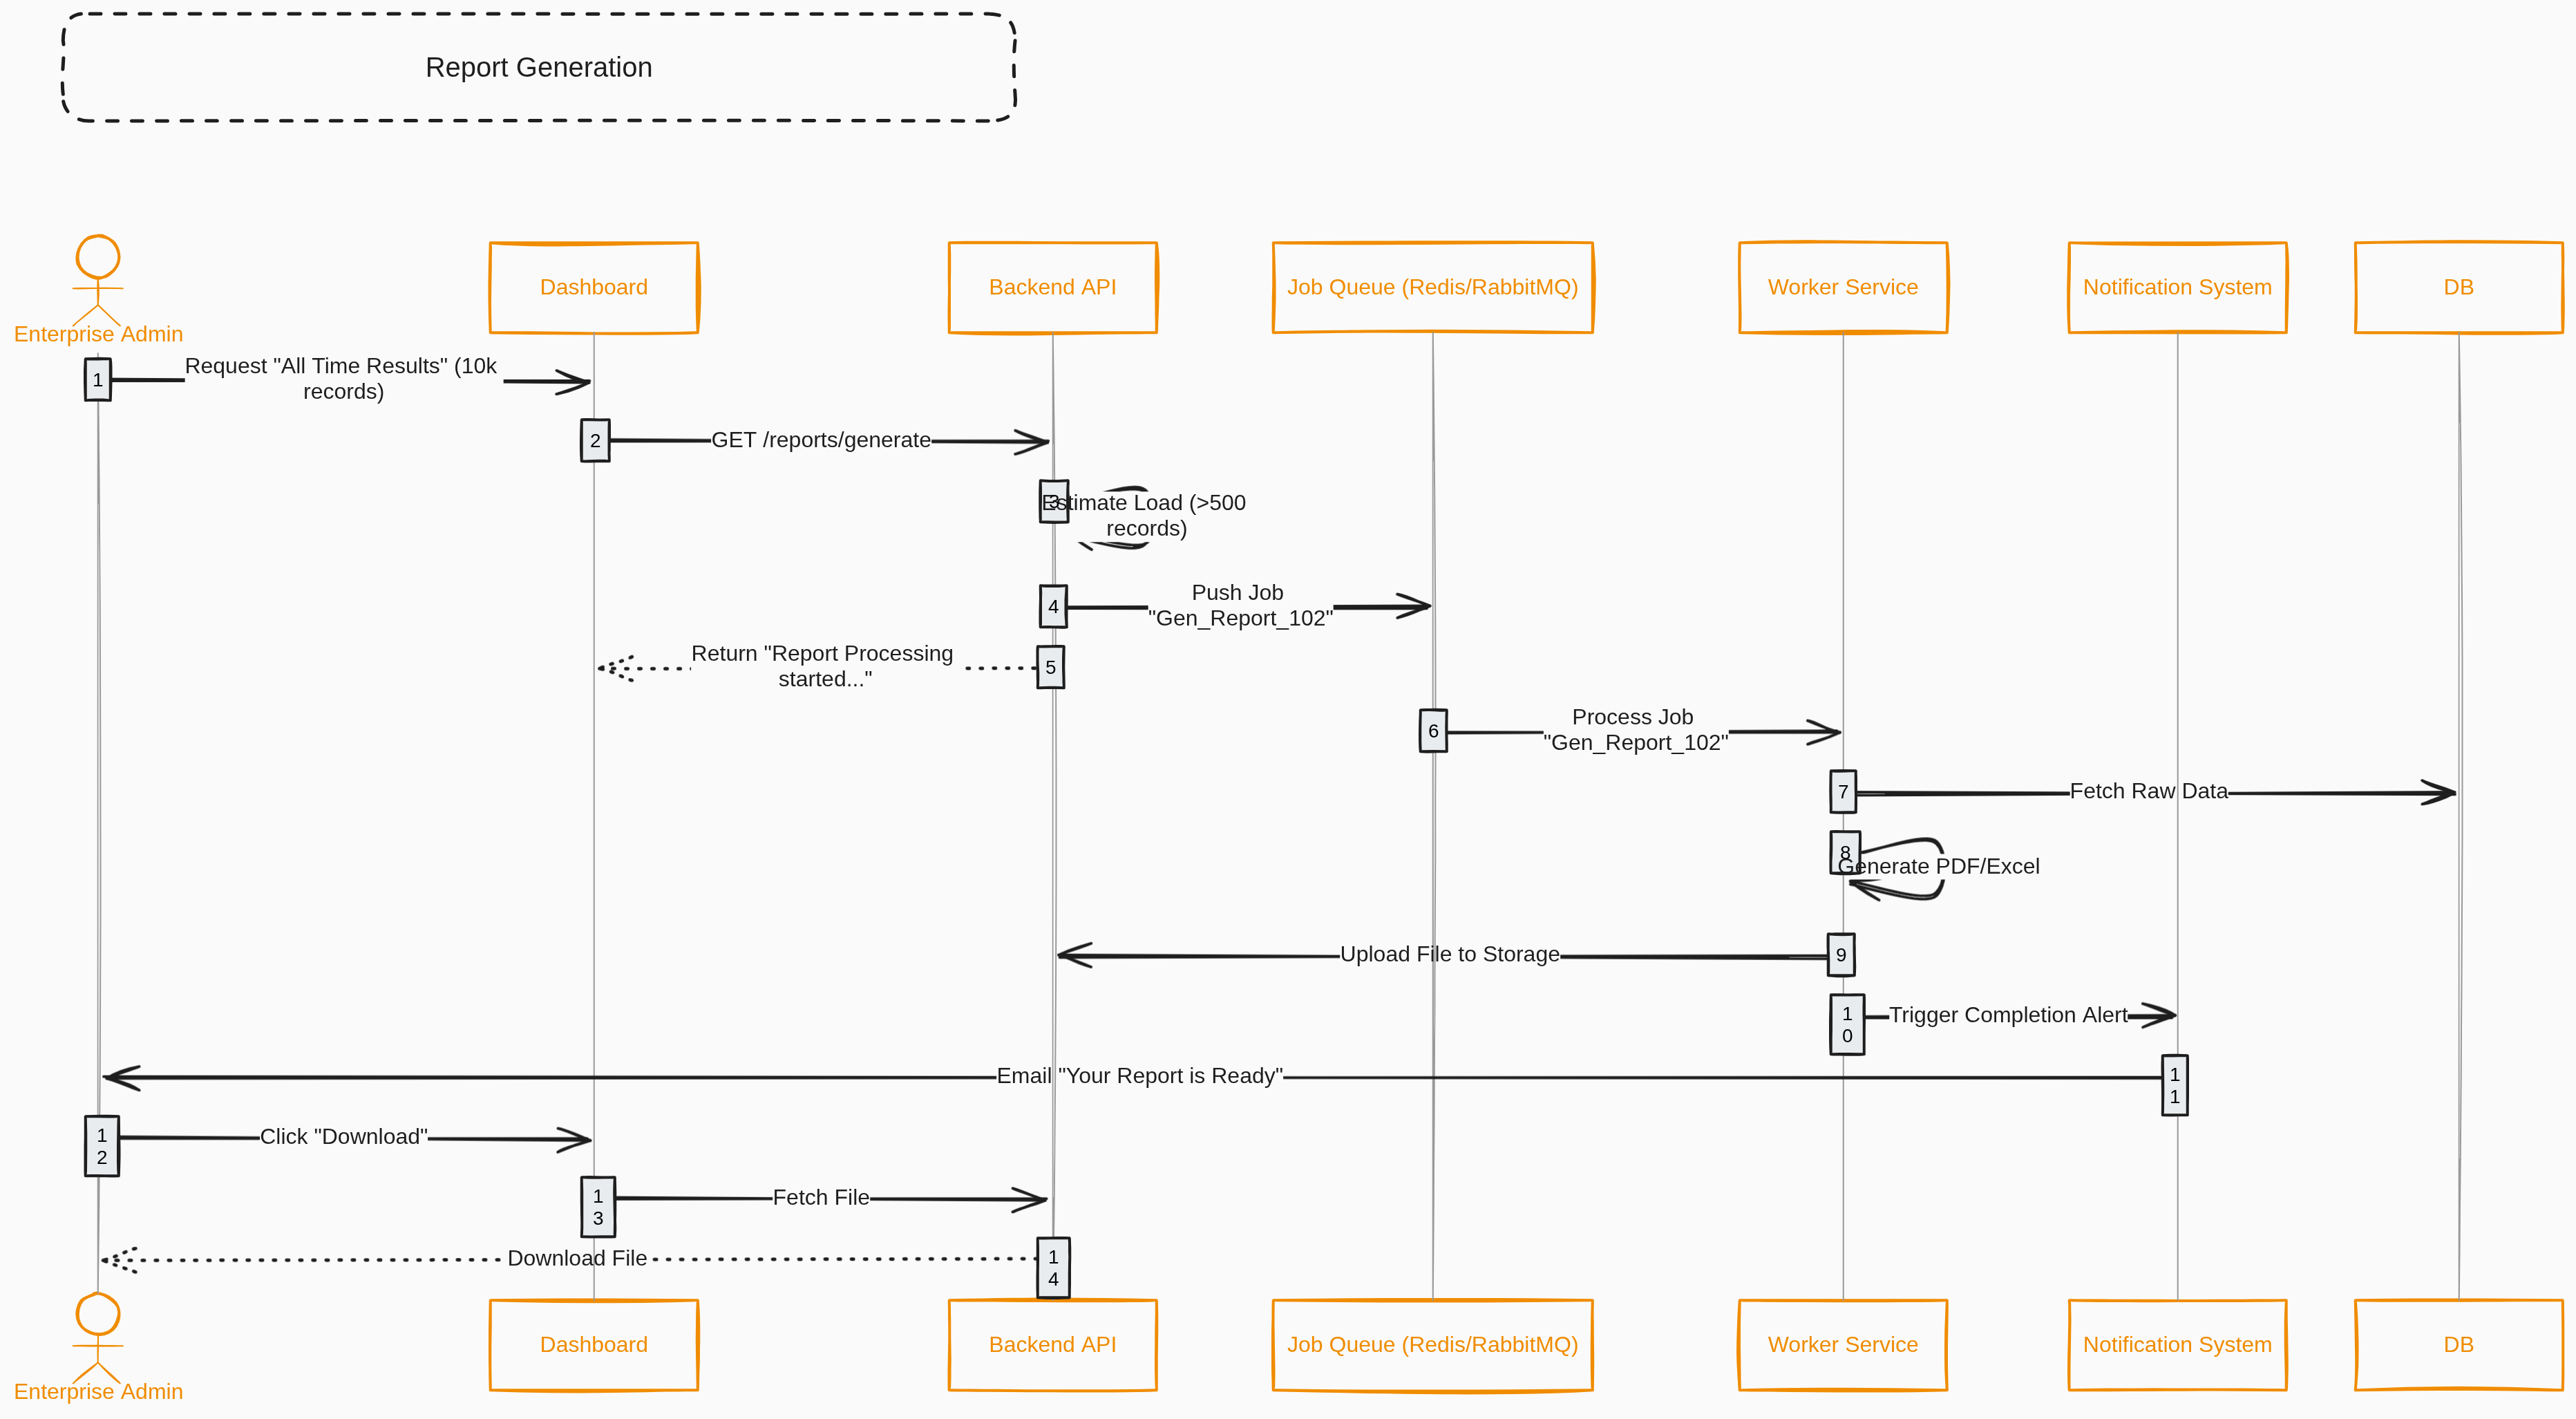
\includegraphics[width=1\linewidth,keepaspectratio]{assets/seq_diagrams/Report Generation.png}
            \caption{Report Generation and Export Sequence Diagram}
            \label{fig:report-generation-export}
            \end{figure}
        \end{itemize}

\end{enumerate}